%Copyright (C) 2021  Geoff Beck
%
%This document is falls under the category of free software: you can redistribute it and/or modify
%it under the terms of the GNU General Public License as published by
%the Free Software Foundation, either version 3 of the License, or
%(at your option) any later version.
%
%This program is distributed in the hope that it will be useful,
%but WITHOUT ANY WARRANTY; without even the implied warranty of
%MERCHANTABILITY or FITNESS FOR A PARTICULAR PURPOSE.  See the
%GNU General Public License for more details.
%
%See https://www.gnu.org/licenses/ for more details

\documentclass[a4paper,10pt,oneside]{book}

\usepackage{fullpage,appendix}
\usepackage{amsmath}
\usepackage{import,url}
\usepackage{tocbibind}
\usepackage[bookmarks=true,plainpages=false]{hyperref}
\usepackage{titletoc}
\usepackage{graphicx}
\usepackage{caption,titlecaps}
\usepackage[a4paper,margin=2cm]{geometry}

\graphicspath{{pictures/}}
\usepackage[T1]{fontenc}
\usepackage{lmodern}


\newcommand{\dicediffbase}{10}
\newcommand{\dicenoprof}{-1}
\newcommand{\dicecritlvl}{4}

\newcommand{\textlf}[1]{\textbf{\titlecap{#1}}}
\newcommand{\textlfirst}[1]{\textbf{\textit{\titlecap{#1}}}}

\title{\textbf{\huge Heroes3D6\\Core Rules}}
\author{Geoff Beck}
\date{}

\begin{document}
\maketitle
\frontmatter
\tableofcontents
\mainmatter

\chapter{Introduction}

\section{Opening Words}
A player's character is their representative in the world of \textit{Heroes3D6} and such should be a personal and fully customisable thing; allowing the player's creativity free reign and not limiting them with too many rules and class attributes etc. This is what \textit{Heroes3D6} tries to do, liberate your role playing experience from restrictive parameters but still maintain some semblance of an ordered and enjoyable system.

\textit{Heroes3D6} depends almost as much on the imagination of the players as it does upon the Game Master. The players are given little or no instruction as to how to fulfil any role within a group and how well they do this will ultimately decide how much fun the game is.

This is a simple system to pick up, as it applies a central set of mechanics across the board, but is complicated enough to please even the most hardcore of gamers, due to the depth and freedom of its mechanics, should you choose to delve into them. The system itself is very open to interpretation and lots of work is required by the Game Master to make this work, as they must make many decisions on the spot as to how the rules apply in a given situation. Other than that, just read and play.

This weighty tome encompasses all the essential rules needed to play a game of \textit{Heroes3D6} independent of setting, other books merely contain rules for playing the game within a famous/iconic world or setting, all these other books require these Core Rules, but do occasionally over-ride them when necessary.

This rule book falls under the category of free software~\footnote{Copyright (C) 2021  Geoff Beck}: you can redistribute it and/or modify
it under the terms of the GNU General Public License as published by
the Free Software Foundation, either version 3 of the License, or any later version (see \url{https://www.gnu.org/licenses/}).

\section{The Core System}
\label{sec:base}

\subsection{Players and the Game Master (GM)}
Games of Heroes are run by a player designated as the Game Master (GM). The remaining participants are simply termed as players. Each of the players controls a character and together they will take part in an adventure supervised by the GM. The Game Master acts as a narrator, they drive the story and is in control of the world and environments inhabited by the player characters. Additionally, they create and control any people or monsters that the characters will encounter in the course of their adventures. 

These rules for the structure of the game are deliberately loose, as the freedom of players and GM to collectively shape an adventure is the magic that makes pen-and-paper role-playing games worthwhile.

\subsection{Actions and Dice Rolls}
An element of randomisation is introduced into the game by the players rolling dice whenever their characters wish to perform non-trivial actions. These rolls tend to be modified by how good the character is at the particular action (making them more or less likely to succeed). Things like breaking down doors, persuading a guard to let you into a locked door, picking a lock, fighting an enemy, noticing someone hiding in the bushes, climbing a tree/wall/ladder/rope, swimming, jumping a gap, riding, or picking pockets are all examples of actions that would require the player to make a roll to see if their character succeeds. 

How good a character is at a particular action is decided by two things, firstly their natural capabilities (Chapter~\ref{chap:attb}) and secondly their learned or acquired skills (Chapter~\ref{chap:skills}). Deciding whether or not a skill or natural attribute is appropriate to a particular task is a matter of common sense and the players and GM can come to a consensus for any contentious tasks. For example: tasks that rely only on the characters strength (actions like breaking things) will not be resolved through skills. However, actions like riding horses, tying or climbing ropes, and picking locks are all things that are greatly enhanced by experience and skill development and thus will rely on skills when resolving such actions. Note that skills still benefit from natural attributes, usually those that give one some advantage in the particular discipline. 

How success and failure are determined is explained in the Section~\ref{sec:rolls} below.

\subsubsection{Dice Notation}
The notation ``requires a 3d6 roll of $16+$'' means that a total score of 16 or greater, on three six-sided dice (3d6), is needed for the given action to succeed. Similarly ``$5-$'' means 5 or less. When no dice code (3d6, 2d6, etc) is given, then 3d6 is considered the default dice set.

\subsubsection{The Opposed Roll and Difficulty Check}
\label{sec:rolls}
The core of this 3d6 system is the \textlfirst{difficulty check}, any task can be assigned a \textlfirst{difficulty} by the Game Master and then is performed successfully if the character scores equal to or greater than the \textlf{difficulty} on a roll of 3d6. To this roll you add the relevant \textlfirst{attribute/skill} score; for instance when making a climbing check you add your athletics score to the roll. The second core mechanic is the \textlfirst{opposed roll}, this represents a contest between two or more opponents, as such each creature contesting the roll adds the given \textlf{attribute/skill} score to a roll of 3d6. The victor is the one whose resultant score is the highest. In the case of a tie, simply roll again.

\subsubsection{Critical Success/Failure}
If you succeed/fail on a check by $\dicecritlvl$ or more you have achieved a \textlfirst{critical success/failure}. For example if you need to beat \textlf{difficulty} 11 to succeed then $15+$ is \textlf{critical success} whereas $7-$ is \textlf{critical failure}. Some effects scale with how many multiples of $\dicecritlvl$ you succeed or fail by.

\subsubsection{Rounding Conventions}
When the division of an integer score results in a non-integer number (i.e. it is not a whole number) then the convention is to round up, unless otherwise specified.

\subsubsection{Edge}
Some circumstances confer great advantage or disadvantage on a character. This is referred to as \textlfirst{edge}. While experiencing an \textlf{edge} bonus while rolling $n$d6, a character rolls $(n+1)$d6 and chooses the highest $n$. In contrast, an \textlf{edge} penalty makes the character roll $(n+1)$d6 dice and choose the lowest $n$. Example: I roll 3d6 to make a check to see if I jump over a crevasse, luckily I have an \textlf{edge} bonus and thus roll 4d6 scoring 3,4,2, and 3. I keep the highest 3 and total 10. If this was an \textlf{edge} penalty I would have totalled 8. 

An \textlf{edge} penalty cancels out a bonus if character is subject to both. If a character has 2 or more \textlf{edge} bonuses/penalties simply add extra dice to the number being rolled. 

\subsection{Heroic Statistics}
Any heroic/villainous character will also posses an attribute called \textlfirst{heroism/villainy}, which can be spent to perform feats of exceptional skill and daring. The central premise of this statistic system is to set heroic characters apart, allowing them to occasionally avoid the vagaries of chance inherent in dice rolling games. 


\section{Useful notes for the GM}
Here we will discuss an important topic: how we assign difficulty scores to feats characters wish to perform. This is non-trivial if you are used to systems that use a single die for rolls, i.e. 1d20 being rolled for skill checks etc. 

\subsection{Assigning difficulties}
The trickiness of difficulty assignment arises from the fact that 3d6 have a non-linear probability distribution, meaning that some scores are far more likely than others. Whereas, on 1d20 every score has an equal chance of occurring. Thus, the GM should be careful, as an increase of 1 difficulty can make a task far more difficult than you would anticipate. To help with this task, I will outline some useful principles in choosing difficulties. The very nerdy reader can look to the appendices for fun things like probability distributions. 

I will divide tasks into 3 groups: easy, moderate, and hard. In order to view these in a vaguely concrete framework, I will sort difficulty scores into these groups assuming there are no bonuses or penalties on the roll. In this situation, a difficulty of lower than 9 is easy, and greater than 13 is rather hard. 

Note that requiring $11+$ on 3d6 is a 50\% probability of success, so this would correspond to something an unskilled character is equally likely to fail or succeed at. A difficulty of $13$ would only imply success 25\% of the time (assuming no bonuses). In contrast, a difficulty of $9$ results in a chance of 75\% of succeeding. These examples should give you sufficient idea of how to assign difficulty. Things that an average man would struggle to achieve should be difficulty $13$ or higher whereas simple tasks can assigned $9$ or lower. In this $9$ to $13$ range each increase or decrease in difficulty by $1$ results in the same probability shift, for lower or higher difficulties the distribution becomes more extreme.




\chapter{Character Attributes}
\label{chap:attb}

A character in \textit{Heroes3D6} is represented by a set of \textlfirst{natural attributes} and their \textlf{heroism/villainy}. The former detail the character's innate abilities while the latter represent their calibre as a potential hero or villain.
Natural attributes are: \textlfirst{might}, \textlfirst{cunning}, \textlfirst{wit}, and \textlfirst{resolve}.

Natural attributes can be used to determine a character's success in certain actions (examples are given in the sections below). As such, success is determined by making a \textlf{difficulty check} with the given attribute.

\section{Natural Attributes}
These reflect the inherent predispositions of the character, based on their personality. There are five attribute statistics and a character's scores are determined following the character creation rules, found in Chapter~\ref{chap:create}. 

\subsection{Attribute Modifiers}
Each attribute contributes to many different skills or activities, its influence on dice rolls is direct, just add it to the result of a relevant roll.

\subsection{Might}
\textlf{Might} is the aggression or assertiveness of the character. A character can make might-checks to, through sheer bloody-mindedness, break objects, bash in doors, or move large objects. The \textlf{difficulty} of breaking objects can be found under the rules for \textlf{Cover}, Section~\ref{sec:cover}, in the Combat rules.\textlf{Difficulty} for lifting or moving heavy objects can be found in Section~\ref{sec:carry} in Baggage and Encumbrance. \textlf{Might} also dictates a character's ability to inflict damage in combat.

\subsection{Cunning}
\textlf{Cunning} is the craftiness of the character. \textlf{Cunning} can be used to bluff convincingly, make feints in combat, trip people up, or get out of the way of harm. It also contributes to the \textlf{stealth}, \textlf{disguise}, \textlf{deceive}, \textlf{slight of hand}, and \textlf{survival} skills. 

\subsection{Wit}
\textlf{Wit} is a character's ability to rapidly adjust to changing circumstances. It affects a character's aim in combat as well as the \textlf{awareness}, \textlf{mechanical}, and \textlf{knowledge} skills. \textlf{Wit} checks would be made if the character had to rapidly assess a situation or react quickly to imminent danger. \textlf{Wit} also decides how difficult it is to deceive or confuse the character. 

\subsection{Resolve}
Is a measure of the character's determination and force of character. \textlf{Resolve} checks can be used to flatter, distract, or to taunt/enrage a target into attacking the character. These checks involve an opposed roll with the target's \textlf{Wit} score. \textlf{Resolve} is also involved in the \textlf{persuade}, \textlf{leadership}, \textlf{healing}, \textlf{insight}, and \textlf{perform} skills. Finally, it regulates a character's ability to resist debilitating effects (magic,drugs,poisons) by pure will. 



\section{Heroic Attributes}
\label{sec:heroism}
\subsection{Heroism/Villainy}
\textlf{Heroism} is what sets your character apart from their more ordinary brethren, it represents a hero's capacity to make decisive and daring actions under pressure. The distinction between \textlf{heroism} and \textlf{villainy} points is one of flavour, villains have \textlf{villainy} while heroes get \textlf{heroism}. Generally, if a rule refers to \textlf{heroism} it still pertains to \textlf{villainy}, unless otherwise stated. 

\textlf{Heroism/Villainy} may be spent to guarantee success on a given action, or to raise the critical success level of a single successful action by 1 (i.e. a success become a critical success and critical success becomes a level 2 critical success). Additionally, \textlf{heroism} may be spent to perform daring feats of valour while \textlf{villainy} may be used for vile trickery; this grants the character access to a single \textlf{perk} of their choice for a few seconds (1 round in combat). There is no need for the character to have bought the chosen \textlf{perk} or have it equipped (it also bypasses limits on \textlf{perk} numbers).

If a character has no \textlf{heroism/villainy} when resting, they may regain 1 point. Otherwise, such points are awarded by the Game Master on the spur of the moment for any deed that is appropriately heroic/villainous. 


\subsubsection{Moment of Glory}
A \textlfirst{moment of glory} awards the character with a single \textlf{heroism/villainy} point they can spend within the next round only.

\subsubsection{Optional rules}
An alternative way to use \textlf{heroism} is to allow characters to make special actions they invent on the spot. The Game Master must decide the consequences of any such actions made.


\section{Perks \& proficiencies}

\textlfirst{Perks} are talents learned or gained by a hero through the course of their adventures, they can be purchased via the expenditure of experience points. A character can have at most 3 active and 3 passive \textlf{perks} equipped at once (only equipped \textlf{perks} can be used). If they know more than 3, they may choose which 3 are equipped. Changing this selection requires an hour's rest and concentration.

\textlf{Proficiencies} are more general skills gained by the character. These are always active and never occupy either passive or active \textlf{perk} equipment slots.
A list of \textlf{perks} and \textlf{proficiencies} can be found in Chapter~\ref{chap:perks}.

\section{Experience points}
Each time the Game Master decides to reward the heroic achievement of a character, or each character in the group, then the relevant characters gain 1 experience point. 
This guideline is very qualitative and this is because heroism is a qualitative thing, so advancement is very much a case of the application of GM judgement, informed by basic guidelines laid down here.

Simple guidelines for experience: a point can be earned by actions demonstrating some heroic calibre, such as: single handedly over-coming many foes or performing reckless feats of strength and daring that save the day. Or perhaps by feats of magic or deeds accomplished through strength of will and force of personality. Experience can also be awarded for devious acts of deceit, or from victory through wit and intelligence rather than blade and boot. Note that these achievements are not combat exclusive, heroism is format-independent after all.

Experience points can be spent on purchasing new \textlf{perks} and \textlf{proficiencies}, the costs of these is detailed in Chapter \ref{chap:perks}. Note that experience cannot be spent in high pressure or active situations, only during periods of rest and contemplation.

\subsection{Advancing Attributes}
Natural attribute points can only be increased in a limited fashion, so choose wisely!



\section{Reputation}
Any hero or villain has a reputation, be it as a magnanimous defender or a scheming thief; so to can characters develop a reputation and even, by great deeds, have their names known and talked of by thousands of admirers/policemen. 

\subsection{Reputation Level}
Reputation is gained by performing important deeds or actions that get you talked about. Saving the mayor's daughter or preventing orcs from killing a group of farmers, that kind of thing. Cheating lots of people out of their money or swindling a local lord or even robbing a bank are also good examples of reputation gaining actions.
Each character has a personal reputation, which is that of the group but modified by personal actions, and the group as a whole has a reputation based on group actions.
Characters start at 0 reputation.

\subsection{Reputation Rating}
This indicates whether your reputation is good or bad, it starts at 0 normally, but depending on your Game Master, it can start at -1 or +1. If you gain reputation for ``bad'' actions you get -1 reputation rating, ``good'' actions get +1, so a negative reputation makes you infamous while positive makes you well-liked.





\chapter{Making a Character}

\label{chap:create}
Simply follow these steps to create a character:
\begin{itemize}
\item
First browse the species available in the campaign setting and choose yourself a species, you may wish to select this based on the modifiers applied to members of that group, or simply on a whim. A default human option would grant you an extra skill for your ``associated skill'' list.
\item
Now select a character \textlfirst{background} from \ref{sec:backgrounds}, or invent one your GM agrees to.
\item 
Select at least one \textlfirst{Conviction} for your character from \ref{sec:convictions} or invent your own.
\item
Select, or invent, the \textlfirst{Flaw} in your character's personality from \ref{sec:flaws} (you may select two at most).
\item
Decide the \textlfirst{goals} that drive your character to pursue adventure.
\item
What \textlfirst{relationships} link the character to other group members, organisations, or people in their past?
\item
Now we come to the most important part of character creation, deciding what kind of person your character is. Use the \textlf{Convictions}, \textlf{flaws} and \textlf{goals} you chose as a skeleton. You need to define a character you are comfortable to play as, but also one who is believable as a real person because, lets face it, its not much of a role playing game if everyone is just a faceless killing machine.
\item
Choose one \textlf{attribute} to have the value 2 and another to be 1, set all other \textlf{attributes} to 0.  Set \textlf{heroism/villainy} to 1. 
\item 
Spend up to 3 experience points choosing \textlf{perks} or \textlf{proficiencies} (Chapter~\ref{chap:perks}) for your character. You may select one weapon proficiency for free.
\item
A character must then choose 2 skills to be \textlf{proficient} in. These skills must be chosen from the ``associated skills'' list for the character's background. 
\item
Now you may select starting equipment, either from a list supplied by the Game Master or from a budget.
\item
Calculate your combat statistics (see Section~\ref{sec:comstat}).
\end{itemize}



\section{Character backgrounds}
\label{sec:backgrounds}
The character's background is their history before adventuring and dictates the set of associated skills they can choose on character creation. Beyond selecting these you should also sketch out a brief back-story for the character, explaining how they fit into the chosen background archetype. You can, of course, add backgrounds appropriate to the setting.

\subsection{Soldier}
The character is a hard-bitten veteran of fighting. Having seen their fair share of blood spilt on the orders of others, they now turn their hand to adventuring instead. Soldier encompasses several possible histories: army conscript, mercenary, city guard, bandit, or gang enforcer. Associated skills: Healing, Survival, Ride, Athletics, Leadership. 

\subsection{Guttersnipe}
The character was born into a life of poverty, scrounging, stealing, and fighting for scraps in back-alleys. This background lends itself to producing street-smart characters who grew up in harsh environments. Such a character is used to being on the wrong side of the law, sometimes even through no fault of their own. Associated skills: Stealth, Slight of hand, Deceive, Insight, Athletics, Awareness.

\subsection{Wanderer}
The character lives the life of a vagrant or vagabond. They move from place to place seeking opportunity, profit, or just thrills. However, many people are suspicious of such a lifestyle and regard the character with suspicion or outright hostility. Wanderer is suited to a character who likes wild places and is resentful or suspicious of petty authority. Associated skills: Survival, Athletics, Stealth, Awareness, Animals, Plants.

\subsection{Silver spoon}
The character was born into old money, nobility, or some similar high social station. They received an expensive education and live an expensive lifestyle. As such these characters are used to political manoeuvrings that go along with high society. Associated skills: Persuade, Deceive, Insight, Leadership, Ride, History, Religion.

\subsection{Professional}
The character has trained long in a craft and has become quite skilled in their own right. This is a broad category and encompass scholars, blacksmiths, engineers, farmers, sailors, and many others. Associated skills: Mechanical, Crafting skills, Awareness, Knowledge skills. 

\subsection{Artist}
The character has trained in the creative arts, being a musician/bard, actor, dancer, sculptor, painter or something similar. Such a character often has a near obsessive devotion to their art form and a tendency to grandiosity. Associated skills: Perform, Athletics, Insight, Persuade, Disguise, History, Religion.

\subsection{Barbarian}
The character is born into a culture deemed savage and backward by most civilised societies (civilisation is often in the eye of the beholder). As such, `sophisticated' individuals tend to view the character with a mixture of terror and revulsion. However, a `barbarian' has their own perspective on what it means to be civil and many valuable skills. Associated skills: Survival, Athletics, Awareness, Ride, Animal, Plant.



\section{Convictions}
\label{sec:convictions}
Convictions are your character's ideals and principles. Their moral code and the truths they believe in. These are suggestions and serve as a guideline for creating your own.

\subsection{Might makes right}
The character believes that strength justifies everything. The weak being preyed upon by the strong is just how the world works. 

\subsection{Nothing for nothing}
The character believes that everything has to be earned, charity only creates dependence.

\subsection{Something for nothing}
The character knows that the destitute need protection, mutual support strengthens everyone. The character believes strongly in charity and doing what they can to help anyone.

\subsection{Words before weapons}
The character will always try to talk before resorting to violence, they are a dedicated pacifist.

\subsection{Kill or be killed}
The character has no qualms about violence and resorts to it often, the non-violent don't last long enough for their principles to matter.

\subsection{Make your own justice}
The law is not be trusted, you have to claim justice for yourself rather than waiting for a court. 

\subsection{The law is the law}
Rules exist for a reason and should be obeyed as closely as possible.

\subsection{Power always corrupts}
No one can be trusted with power. All authority should be looked upon with suspicion as the powerful are the enemy.

\subsection{The ruled need rulers}
People are sheep and need a shepherd. Conveniently, you are just the person for the job.

\subsection{Serve a greater good}
There are things more important than any one individual, such a cause drives your actions (make up a suitable one).

\subsection{Knowledge is power}
Knowledge is vital, curiosity and the drive to learn are fundamental to civilisation. The character will always aim to ferret out secrets.

\subsection{Honour is paramount}
You cannot control how others behave but you can always choose to do the right thing. The character assiduously follows a code of honour (make up a suitable one).



\section{Flaws}
\label{sec:flaws}
Flaws are what make your character the imperfect creature they are. These are suggestions and serve as a guideline for creating your own.

\subsection{Jenkins}
The character is impulsive and will not hesitate to act while their comrades debate the best course of action.

\subsection{Clumsy}
The character is not the sharpest tool in the shed, in fact you will be lucky if they don't burn the shed down by accident while searching for tools.

\subsection{No Diplomat}
The character has a habit of saying the first thing to come into their head, regardless of how inappropriate it is to the current situation (they may not take the Diplomat perk either).

\subsection{Dipsomaniac}
The character is a borderline addict to a chosen substance and will go out of their way to consume it.

\subsection{All about Me}
Such a character will see themselves as the centre of events at all times and will seldom acknowledge the efforts and contributions of others. This can manifest in anything from a tendency to self-importance to a narcissistic view that any praise is their due and any criticism levelled against them is out of pure jealousy. 

\subsection{Better with Animals}
This character is a rough soul who prefers life in the thick of nature to a bustling city. As such they tend to be a bit brusque with ``soft'' city dwellers and contemptuous of petty authorities like watchmen and mayors.

\subsection{In It to Win It}
The character takes competitive to the extreme, and has to be the best at everything they do. Their pride is greatly wounded when this is not the case. 

\subsection{Driven}
The character has a guiding obsession that they will seek to pursue regardless of more pressing matters (pick a suitable obsession).

\subsection{Scarred}
The character has been both mentally and physically scarred by exposure to violence or trauma. This may manifest as anything from flash-backs or violent outbursts, to long boring stories about events of the character's past. The severity can be chosen based on the character's history.

\subsection{Out of Touch}
The character is absorbed in day dreams and speculation, often being more concerned with knowledge and thought than real events. As such, the character tends to appear forgetful and oblivious and can often cause touchy individuals to take offence (as they might feel ignored).

\subsection{Money grubber}
The character is greedy and always looks to profit regardless of the situation.

\subsection{Temper temper}
The character angers quickly and is prone to outbursts of anger when pushed.

\subsection{Arrogant}
The character is assured of their superiority to others and is often condescending.

\subsection{Paranoid}
The character sees a conspiracy in every shadow and a threat around every corner. They would sleep in full plate if they could.

\subsection{Too trusting} 
The character can't help but expect others to be as nice as they are. Thus, they implicitly trust everyone who doesn't seem outrageously shifty.

\subsection{Domineering}
The character is used to getting their own way. They don't take questioning of their authority well, expect everyone to do their bidding, and may be unwilling to listen to the ideas of others.

\subsection{Touchy}
The character has a sense of pride that can be easily bruised. They feel the need to have their usefulness affirmed often.

\subsection{Master debater}
The character can't help but argue. They will challenge any assertion they can and will pursue arguments relentlessly.



\section{Relationships}
\label{sec:relationships}
These are your character's links to other people or places, it is often sensible to select relationships that link your character to at least one other in the adventuring group. These can be things like old friends, family links, or an organisation that your character is part of or linked to. This can be a powerful tool for making your character a part of the world you adventure in, so it should be carefully considered.


\section{Goals}
\label{sec:goals}
Everyone has an ambition, something that motivates them to wake up every morning. Goals are what motivate your character to adventure. These can be things like fame, riches, public office, honours, or secret knowledge. Other suggestions could be revenge or the finding of lost friends/relatives. Think about choosing your goals as selecting an initial objective for your character, an opening arc to their story.




\chapter{Character Skills}
\label{chap:skills}
There are several skills available to aid your progress through adventures.

\section{Skill proficiency}
\label{sec:skill-prof}
If a character is \textlf{proficient} with a given skill then they add the synergy attribute to associated rolls. This attribute usually follows the skill name. Otherwise, they add -1. A character can either be trained in a skill (requires 20 hours of training) or spend 3 experience to gain proficiency.


\section{Using a Skill}
\label{sec:use-skill}
A skill check is made whenever it is deemed appropriate by the Game Master, for instance an athletics check must be made when a character wishes to jump over a precipice or to climb up a building. Further examples of when skills might be used are listed in their descriptions in following sections.

When using a skill the character must exceed the \textlf{difficulty} of the task on a roll of 3d6, adding either their synergy attribute or -1. The \textlf{difficulty} of a task is at the Game Master's discretion. If the roll equals or exceeds the required \textlf{difficulty} score, then a \textlfirst{success} is achieved. However, if the roll exceeds the \textlf{difficulty} by $\dicecritlvl$, or more, a \textlf{critical success} is achieved. Failing a check by $\dicecritlvl$ or more results in \textlf{critical failure} (with suitably enhanced consequences chosen by the GM). Note that the advantages/penalties of \textlf{critical success/failure} should scale with the number of multiples of $\dicecritlvl$ by which the role exceeds/fails the \textlf{difficulty}. 

\subsection{Failure and Pressure}
If there is no consequence to failure, a character may claim success without rolling. If they roll instead, they have an \textlf{edge} bonus but must accept the result. 

\subsection{Multi-stage checks}
\label{sec:multi-stage-skills}
Sometimes a character wishes to accomplish a long and daunting task. Some examples might be swimming across a lake/wide river, climbing a cliff, galloping over rocky ground on a mount, or following tracks. To represent this the GM should choose to split the task up into two or three separate checks. To complete the task the character must achieve a matching number of successes. The bullet-point list below explains how each check should be made. The ``unpleasant consequence'' should be appropriately chosen, i.e. drowning when swimming, falling off when climbing, etc. 
\begin{itemize}
	\item Make a check
	\item Success means the check is complete
	\item \textlf{critical success} by-passes the next check as well
	\item Failure means you must re-try
	\item \textlf{critical failure} results in some unpleasant consequence
\end{itemize} 

\section{Skill List}
Here are some sample skills, each setting/world may add or remove from this list as appropriate.

\begin{table}[ht!]
	\centering
	\caption{Skills (synergy attributes in brackets)}
	\begin{tabular}{|l|l|l|}
		\hline
		 General & Social & Knowledge\\ [0.5ex]
		\hline
		Athletics (M) & Perform (R) & Animals (W)\\
		Slight of Hand (C) & Leadership (R) & Plants (W)\\
		Awareness (W) & Deceive (C) & History (W)\\
		Stealth (C) & Disguise (C) & Religion (W) \\
		Healing (R)  & Persuade (R) & Arcana (W)\\
		Mechanical (W)  & Insight (R) & \\
		Ride/Drive (C) & & \\
		Survival (C) & & \\
		Alchemy (C) & & \\
		\hline
	\end{tabular}
\end{table}



\section{General Skills}

\subsection{Alchemy/Chemistry (Cunning)}
Alchemy/chemistry is the craft of mixing chemicals and ingredients to brew potions or create useful compounds. Whether it is creating mixtures to achieve almost miraculous effects, or simply mistakes that produce spectacular explosions, the chemist can whip up a potion to suit any need.

Creating a chemical brew requires suitable ingredients of course (this is up to the Game Master but try make them sensible, like an ogre's tooth for a strength potion, appropriate steroids for an adrenal stimulant; that kind of thing). A chemical draft also needs a container and generally a set of glass vessels and equipment for measuring, grinding and heating ingredients (chemist's tools) that can be purchased from an chemist or supplier of specialist equipment.

\textlf{Critical success} adds one extra output item produced per critical level. \textlf{Critical failure} ruins 1 extra set of materials per critical level.

\subsection{Healing (Resolve)}
A healer is one who is skilled is speeding the recovery of their allies through strictly medical/surgical means (potions are the province of the chemist), a healer can employ their healing skill to remove injuries inflicted to an ally. You may only ever make 1 re-attempt on a failed healing roll, should this also fail, you may not re-attempt to heal that particular patient in the same day. The kind of healing actions are:

\begin{itemize}
	\item Cure a single \textlf{wounded} effect
	\begin{itemize}
		\item \textlf{difficulty}: $\dicediffbase$ (add 1 extra for each other wound effect present)
		\item Failure means nothing changes
		\item \textlf{Critical failure} increases healing difficulty for that target by 1 for 3 days
		\item \textlf{critical success} removes an extra wounded effect per critical threshold, or badly-wounded per two thresholds instead
	\end{itemize}
	\item Cure a single \textlf{badly wounded} effect
	\begin{itemize}
		\item \textlf{difficulty}: 12 (add 1 extra \textlf{difficulty} for each additional wound effect present)
		\item Failure means nothing changes
		\item \textlf{Critical failure} increases healing difficulty for that target by 1 for 3 days
		\item \textlf{critical success} removes an extra wounded effect per critical threshold, or badly-wounded per two thresholds instead
	\end{itemize}
	\item Cure a single \textlf{Mortally wounded} effect
	\begin{itemize}
		\item \textlf{difficulty}: 15 (add 1 extra \textlf{difficulty} for each additional wound effect present)
		\item Failure means nothing changes
		\item \textlf{Critical failure} increases healing difficulty for that target by 1 for 3 days
		\item \textlf{critical success} removes an extra wounded effect per critical threshold, or badly-wounded per two thresholds instead
	\end{itemize}
	\item Identify poison or disease
	\begin{itemize}
		\item The difficulty should scale with the rarity of the condition or the healers familiarity with it
		\item Failure means the healer doesn't know
		\item \textlf{Critical failure} means they get it wrong
	\end{itemize}
	\item Analyse wounds (what caused them etc)
	\begin{itemize}
		\item The difficulty should scale with the rarity of the type of creature/weapon or the healers familiarity with it
		\item Failure means the healer doesn't know
		\item \textlf{Critical failure} means they get it wrong
	\end{itemize}
\end{itemize}


\subsection{Athletics (Might)}
This skill determines your ability perform acrobatic feats, swim, climb, jump long distances or keep your balance. Any task of this nature is given a difficulty score by the Game Master, the degree of success or failure should be noted by the Game Master for purposes of describing your heroic leap or clumsy stumble into a precipice.  This skill can be used to:

\begin{itemize}
	\item Climb
	\begin{itemize}
		\item Difficulty should scale with available hand-holds and height of the climb
		\item A short climb should require only one success
		\item Longer climbs should be multi-stage checks (see \ref{sec:multi-stage-skills})
		\item Climb speed is increased by \textlf{critical success}
		\item Failure results in pausing the climb to get better grip, must re-try to continue
		\item \textlf{Critical failure} results in falling off
	\end{itemize}
	\item Jump long distances (more than half body height)
	\begin{itemize}
		\item Difficulty should scale with distance (e.g. 7 for half height, 11 for full height)
		\item Add 2 for vertical jumps
		\item Failure means the jumper falls short (potentially into a crevasse)
		\item Additionally, \textlf{Critical failure} by X thresholds results in the jumper suffering X damage rolls. These hits have \textlf{power} 0.
	\end{itemize}
	\item Swim long distances or in difficult waters
	\begin{itemize}
		\item Difficulty should scale with how rough and deep the water is (7 for still, 16 for a flowing torrent)
		\item A short swim should require only one success
		\item Longer swims should be multi-stage checks (see \ref{sec:multi-stage-skills})
		\item \textlf{Critical success} increases swim speed 
		\item Failure results in struggling to stay afloat, must re-try to continue
		\item \textlf{Critical failure} by X thresholds means the character must pass a \textlf{Resolve} check with difficulty $\dicediffbase$ + X or drown. 
	\end{itemize}
\end{itemize}

\subsection{Stealth (Cunning)}
Stealth has two functions: to move about unnoticed or to conceal yourself while stationary. Thus, this skill can be used to:

\begin{itemize}
	\item Move silently without being noticed
	\begin{itemize}
		\item Opposed roll vs any observers \textlf{awareness} skill
		\item Bonuses may be gained by being in cover (see Table~\ref{tab:cover}) and an \textlf{edge} bonus is granted by being in shadows
		\item Success means you are undetected
		\item \textlf{critical success} grants you \textlf{edge} on your next \textlf{stealth} check
		\item Failure results in potential observers searching for you (you can try hide from them)
		\item \textlf{Critical failure} additionally incurs an \textlf{edge} penalty on subsequent hide checks
	\end{itemize}
	\item Hide and avoid being noticed
	\begin{itemize}
		\item Opposed roll vs the highest \textlf{awareness} skill of anyone trying to find you
		\item Bonuses may be gained by being in cover (see Table~\ref{tab:cover}) and an \textlf{edge} bonus is granted by being in shadows
		\item Success means you are undetected
		\item \textlf{critical success} grants you \textlf{edge} on your next \textlf{stealth} check
		\item Failure means searchers notice your presence
		\item \textlf{critical Failure} results in being noticed (but you don't realise this)
	\end{itemize}
\end{itemize}

\subsection{Awareness (Wit)}
Is how observant and alert a character is, this skill allows you to spot secret doors and notice hidden enemies or traps. This skill can be used to:

\begin{itemize}
	\item Search an area for concealed objects/people
	\begin{itemize}
	\item \textlf{difficulty} for an object is decided by the Game Master. Otherwise see \textlf{stealth}.
	\item Success means you notice the object or creature while you search
	\item The amount of detail revealed should scale with the number of critical thresholds the \textlf{difficulty} is exceeded/failed by
	\item \textlf{Critical success} also means a searched for creature doesn't detect that they have been spotted
	\item \textlf{Critical failure} grants an \textlf{edge} penalty on subsequent checks
	\end{itemize}
\end{itemize}


\subsection{Mechanical (Wit)}
Mechanical skill represents how mechanically minded a character is, allowing them to build, modify, sabotage or disable mechanical devices such as traps or siege weapons. A character can use this skill to:

\begin{itemize}
	\item Repair broken mechanisms 
	\begin{itemize}
		\item \textlf{difficulty} should be based on the complexity of the machine being worked with
		\item Success allows you to get the device working temporarily (for 30 seconds or so)
		\item \textlf{critical success} means the mechanism is fully repaired
		\item Failure means that parts will need to be replaced to fix the mechanism
		\item \textlf{Critical failure} results in the mechanism being permanently broken
	\end{itemize}
	\item Disable mechanisms
	\begin{itemize}
		\item \textlf{difficulty} should be based on the complexity of the machine being worked with
		\item Success allows you to disable the device temporarily (for 30 seconds or so)
		\item \textlf{critical success} means the mechanism can be disabled as long as you wish
		\item Failure means that device remains active
		\item \textlf{Critical failure} results in the mechanism being triggered
	\end{itemize}
	\item Pick locks
	\begin{itemize}
		\item \textlf{difficulty} should be based on the complexity of the lock being worked with
		\item Success allows you to open the lock but it is obvious it was picked (scratches, damage etc)
		\item \textlf{critical success} means the picking left no trace
		\item Failure means that the lock remains locked
		\item \textlf{Critical failure} results in breaking a lock pick
	\end{itemize}
\end{itemize}

\subsection{Ride/Drive (Cunning)} 
This skill governs how well the character deals with mounts and/or vehicles. The skill can be used to:
\begin{itemize}
	\item Stay mounted moving through rough or dangerous terrain (see Section~\ref{sec:terrain}) 
	\begin{itemize}
		\item Difficulty 8 - 12 (rough) and 11 - 16 (dangerous)
		\item Frequency of such checks should depend on speed, walking speed makes this unnecessary
		\item Over longer distances use multi-stage checks (see \ref{sec:multi-stage-skills})
		\item \textlf{Critical failure} means a dismount plus the rider suffering X damage rolls, where X is the number of critical thresholds failed by. These hits have \textlf{power} 0.
	\end{itemize}
	\item Execute special manoeuvres that might risk being dismounted while moving
	\begin{itemize}
		\item \textlf{difficulty} should be based on how complex the manoeuvre is (7 is easy, 16 is very very hard)
		\item \textlf{Critical success} grants an \textlf{edge} bonus to associated actions
		\item Failure results in completing the manoeuvre and falling off
		\item \textlf{Critical failure} additionally results in the rider suffering X damage rolls, where X is the number of critical thresholds failed by. These hits have \textlf{power} 0.
	\end{itemize} 
	\item Make ranged weapon attacks while mounted
	\begin{itemize}
		\item \textlf{difficulty} should be determined by the speed and bumpiness of the motion
		\item \textlf{Critical success} grants an \textlf{edge} bonus to \textlf{Aim} 
		\item Failure incurs an \textlf{edge} penalty on \textlf{aim}
		\item \textlf{Critical failure}, by X thresholds, results in being dismounted and automatically failing the damage rolls of X projectiles
	\end{itemize}
\end{itemize}
For additional mounted combat rules see Section~\ref{sec:mountandblade}.


\subsection{Survival (Cunning)}
Survival covers wilderness survival skills, knowing the signs to follow to find water, being able to track animals or people and knowledge of shelter-building. 

\begin{itemize}
	\item Follow tracks
	\begin{itemize}
		\item Low difficulty for soft ground and distinctive marks, high difficulty in hard ground or in a busy location
		\item Success keeps you on the trail, longer trails should be multi-stage checks (see \ref{sec:multi-stage-skills})
		\item \textlf{critical success} means you can rapidly follow the trail
		\item Failure means you lose the trail but can try again
		\item \textlf{critical failure} means you lose the trail entirely
	\end{itemize}

	\item Find water
	\begin{itemize}
		\item \textlf{difficulty} based on water abundance in area
		\item Success means you find a water source
		\item Failure means you find nothing
		\item \textlf{critical failure} you find contaminated water but don't realise this
	\end{itemize}

	\item Tame a wild creature (or calm a frightened creature)
	\begin{itemize}
		\item \textlf{difficulty} determined by wildness/fright-level
		\item Success calms a creature down 
		\item \textlf{critical success} needed to tame a wild creature
		\item Failure means the animal stays wary/frightened
		\item \textlf{critical failure} means the animal bolts or attacks (as appropriate)
	\end{itemize}

	\item Command a tamed creature
	\begin{itemize}
		\item \textlf{difficulty} ranges from 7 for an action the animal would perform of its own volition, to 18 for something that would be totally opposed to the animal's nature or obviously highly risky for the animal
		\item Success means the command will be followed
		\item \textlf{Critical success} grants the creature \textlf{edge} on commanded actions
		\item Failure results in refusal to obey
		\item \textlf{Critical failure} results in the beast attacking or bolting (as appropriate)
	\end{itemize}
\end{itemize}



\subsection{Slight of Hand (Cunning)}
This skill is related to the character dexterity, it covers the ability to perform simple actions quickly without attracting notice. This skill can be used to:

\begin{itemize}
	\item Perform conjuring tricks
	\begin{itemize}
		\item Opposed roll against the audience's collective \textlf{wit}
		\item Success completes the trick impressively
		\item \textlf{Critical success} could allow a additional skill action like picking an audience member's pockets
		\item Failure results in the trick being unimpressive
		\item \textlf{Critical failure} results in the audience seeing how the trick is being done
	\end{itemize}
	
	\item Pick pockets
	\begin{itemize}
		\item Opposed roll against the victim's \textlf{wit}
		\item Success acquires one item from pocket
		\item \textlf{Critical success} allows an extra item to filched
		\item Failure results in the character acquiring nothing
		\item \textlf{Critical failure} results in being detected by the victim
	\end{itemize}
	
	\item Take or exchange items unnoticed
	\begin{itemize}
		\item Opposed roll against highest potential observer's \textlf{wit}
		\item An \textlf{edge} penalty is applied if the item is being actively guarded
		\item Success completes the task unnoticed
		\item \textlf{Critical success} means the theft/replacement won't be noticed for some time
		\item Failure results in the character acquiring nothing
		\item \textlf{Critical failure} results in being detected
	\end{itemize}
\end{itemize}


\section{Social skills}

\subsection{Perform (Resolve)}
This skill represents practice and talent in some form of performance, be it poetry, acting, song, or playing music. A character with this skill can perform their art by rolling this score opposed to the \textlf{difficulty} of the performance they are attempting, this \textlf{difficulty} is related directly to the beauty or skill of the performance. If a character seeks to perform with an instrument they have no experience with, they suffer an \textlf{edge} penalty on perform checks with the unknown instrument.

A general guideline would be that an ``average-joe'' performance has difficulty 8, but no one would pay to watch this.

The amount of audience appreciation/fruit-throwing also scales with the number of critical thresholds the \textlf{difficulty} is exceeded/failed by. 


\subsection{Disguise (Cunning)}
This skill represents your character's ability to obfuscate their appearance, using carefully chosen clothing, make-up or apparatus like moustaches and wigs.  To use the skill you do the following
\begin{itemize}
	\item Concoct your disguise
	\item The GM assigns \textlf{edge} penalties or bonuses as appropriate (based on how well the disguise could work) 
	\item Make a \textlf{disguise} check and record the score
	\item An observer makes an \textlf{awareness} check against your recorded score
	\item If they fail they are fooled by the disguise
	\item If they succeed they are suspicious
	\item Their \textlf{critical success} means they see through you immediately
\end{itemize}  

\subsection{Persuade (Resolve)}
This is a skill that can be used to weedle favours out of people, convince them of your trustworthiness (or some other fact), and for bargaining and bartering. This skill cannot be used to convince a person of something that is untrue (you can't lie while using it).
\begin{itemize}
	\item In ordinary conversation
	\begin{itemize}
		\item Formulate your persuasive words and/or actions
		\item The GM assigns \textlf{edge} penalties or bonuses as appropriate (based on how well this could work)
		\item Make your \textlf{persuade} check opposed to the target's \textlf{wit}
		\item Success means they are convinced
		\item \textlf{critical success} means they also regard you trustingly
		\item Failure means they are dubious
		\item \textlf{critical failure} means they are now suspicious of your intentions
	\end{itemize}
	\item In combat to intimidate enemies (1 action point)
	\begin{itemize}
		\item Formulate your intimidation
		\item Opposed roll versus target's \textlf{wit}
		\item Success means target suffers \textlf{edge} penalty to rolls linked to next action
	\end{itemize}
\end{itemize}


\subsection{Deceive (Cunning)}
This is a skill that can used to lie convincingly, it works in the same way as \textlf{Persuade} but relies on the fact that you are persuading the target of something you do not believe is true, or making a bargain that is not what the target believes it to be (selling them a fake or stolen artwork for instance).

\subsection{Leadership (Resolve)}
Leadership gauges the character's ability to inspire others to follow them, or to bring out the best in each of their companions. This skill can only be used on creatures who can understand you. This skill can be used to:

\begin{itemize}
	\item Make a creature ``snap out of it''
	\begin{itemize}
		\item This negates a condition affecting a target
		\item The allowed conditions: \textlf{Stagger}, \textlf{Crippled}, \textlf{Immobilized}, \textlf{Knock-down}.
		\item The \textlf{difficulty} is given by $\dicediffbase +$ the \textlf{power} of the condition 
		\item \textlf{Critical success} allows you to use this action again for no action points
	\end{itemize}

	\item Direct an action 
	\begin{itemize}
		\item Give an order to an ally
		\item Make an opposed check with your \textlf{Leadership} vs \textlf{difficulty}
		\item \textlf{difficulty} determined by the directed action
		\item If you succeed, and the ally obeys, the action has an \textlf{edge} bonus
		\item \textlf{Critical success} grants an extra \textlf{edge} bonus per threshold
	\end{itemize}

	\item Command and be obeyed
	\begin{itemize}
		\item Issue a single sentence command to a target
		\item If you win an opposed check with your \textlf{Leadership} vs a chosen target's \textlf{Resolve} they obey the command
		\item Target's cannot be overtly hostile for this to work and must be able to understand the command
		\item \textlf{Critical success} grants an \textlf{edge} bonus to the next command to the same target
		\item \textlf{critical failure} means they have \textlf{edge} versus further orders
	\end{itemize}

	\item Restore \textlf{endurance} to others
	\begin{itemize}
		\item Choose a single ally to inspire
		\item Make \textlf{Leadership} check against $\dicediffbase$ + target's missing \textlf{endurance}
		\item Success restores 1 missing \textlf{endurance}
		\item \textlf{Critical success} restores extra \textlf{endurance}.
	\end{itemize}
\end{itemize}

\subsection{Insight (Resolve)}
Is how well a character can read the motives and feelings of others. This skill can be used to:

\begin{itemize}
	\item Determine someone's motives 
	\begin{itemize}
		\item Opposed roll versus target's \textlf{deceive} skill (if they are deceptive)
		\item Otherwise \textlf{difficulty} is decided by how obvious their motives are
		\item The amount of detail revealed should scale with the number of critical thresholds the \textlf{difficulty} is exceeded/failed by
	\end{itemize}
	\item Detect deception 
	\begin{itemize}
		\item Opposed roll versus target's \textlf{deceive} skill
		\item Success means you identify if the person is hiding something
		\item The amount of detail revealed should scale with the number of critical thresholds the \textlf{difficulty} is exceeded/failed by
	\end{itemize}
\end{itemize}



\section{Knowledge skills}
All of these skills follow a similar template.

\subsection{Knowledge (Wit)}
This represents the character's knowledge about a given subject area. It can be used to:

\begin{itemize}
	\item Recall information
	\begin{itemize}
		\item \textlf{difficulty} given by how obscure the subject is
		\item Degree of success determines how much is remembered
		\item \textlf{critical failure} can result in incorrect remembering
	\end{itemize}
	\item Identify objects and properties
	\begin{itemize}
		\item \textlf{difficulty} given by how obscure the subject is
		\item Degree of success determines how much is remembered
		\item \textlf{critical failure} can result in incorrect identification
	\end{itemize}
\end{itemize}


%\chapter{Social interactions}
%\label{chap:social}
%
%This is a short chapter that outlines the rules for social interactions that are transactional in nature. This means these rules apply if the player and/or npc have something they wish to obtain from the interaction (be it information, help or material reward). 
%
%\section{A round of discussion}
%A social interaction is divided into rounds. Each round has consists of two phases, a proposition-reply phase which is followed by resolution. 
%
%\section{Motivations}
%This kind of interaction has an objective, one or both parties want to obtain something or at least not to give something up. If this is clear cut then this forms the relevant motivation. If one party does not have an obvious motivation we instead consider their character traits and what they would generally desire (fame, wealth, etc). Motivations are vital because they decide how effective a given attempt at persuasion or deception is (a selfish character is unlikely to be motivated by the idea he would be doing a good deed for instance).
%
%\section{Proposition and reply}
%The character with advantage (or, in the first round, the one who initiated the discussion) makes a proposition choosing what they will say and selecting the relevant skills. Once this has been stated the other character makes a reply while selecting relevant skills.  
%
%\subsection{Relevant skills} 
%If a party in the discussion is not using just his \textlf{Resolve} then he can choose a relevant skill. \textlf{Persuade} or \textlf{deceive} can always be considered relevant. However, in some circumstances other skills can be relevant too, for instance if persuading someone you are skilled enough to achieve a particular goal, or confusing them with technical jargon. If the skill is not obviously relevant you must persuade the GM of this.
%
%\section{Resolution} 
%If the replying party agrees to the proposition then discussion is over and the proposer has achieved his desired objective. Otherwise, \textlf{opposed rolls} are made between the parties and this ends the round. The GM must apply bonuses/penalties to the parties according to the following considerations: does the choice of words and relevant skills line up with the target's motivations? Sometimes this means an automatic failure can occur. For instance if you attempt to offer someone 100 g to kill themselves this will fail regardless of how charming you are. An example of a poor choice would be trying to convince a target who distrusts experts based on a technical explanation using your engineering skill. The same target could instead have his ego flattered and this would be more effective. It is suggested the DM apply \textlf{edge} bonuses/penalties first before resorting to numerical adjustments. 
%
%The winner of the round now has advantage, and unless this ends the discussion, a new round starts.
%
%\section{Ending a discussion}
%If a party succeeds two rounds in a row they win the discussion and obtain their objective, otherwise the discussion ends if agreement is reached. \textlf{Critical failure} immediately ends the discussion with no winner (unless it is more appropriate that the other participant wins in this case). \textlf{Critical success} wins the discussion immediately. A party can also elect to leave the discussion at any time. (The GM can use this if players try to repeat the same persuade roll more than once as the target has already refused). 
%
%\section{Example discussion}
%In this example we have character persuading a nobleman's servant to let him copy the manor-house key. The character wants the key and the servant does not want to be in position to be caught doing this, but is tempted by avarice. The character selects just to try persuade skill and says ``Look, its a few gold in your pocket, your family could use that, the key will be back after an hour; no one will know''. The peasant replies ``little good a few gold will do me and mine if I get caught''. \textlf{Opposed rolls} are made and the servant wins. He now has advantage and round 2 begins. The servant is the proposer now and says ``but, if you can promise it won't find it's way back to me, and throw in a few more gold...''. The character can now choose to either just reassure the servant and pay extra, or also try talk the price back down. He elects just to take the extra cost and say ``of course, you don't have the only key, no way anyone would know''. Rolls are made with an \textlf{edge} bonus because he acceded to the demands of the avaricious servant. The character achieves a success. The discussion ends as the parties have come to an agreement. 




\chapter{Combat}
\label{chap:combat}
Combat is divided into rounds, each combatant has a chance to act during each round. This chapter covers all the factors that influence combat and detail the normal actions that may be performed during the fighting.

\section{Combat Structure}
Combat is typically a battle between two opposed sides. Both sides will declare actions/intentions first. After this, which side acts first will be determined and then that side's actions are all resolved at the same time.  

\subsection{Action Points}
Action points are the basic currency of combat, each combatant has two available per round. Most actions cost 1 point, however, some cost 2 points or more. A cost of 3 or more indicates that it takes more than 1 turn to finish the action.

\subsection{Action Declaration}
At the beginning of a round of combat each fighter declares what action they intend to make this round (go clockwise from the GM for instance). A fighter may not declare actions in response to other declarations (as this information exists only within the mind of each fighter). Once all fighters have declared their intended actions, the combat moves on to initiative and action resolution. Fighters must spend action points to declare their actions.

\subsection{Initiative}
Each side rolls a single 1d6, the higher score has the initiative and will have their actions resolve first. In the case of a tie, simply resolve everything at once.

\subsection{Action Resolution}
For the side with the initiative, each fighter gets a chance to make their declared actions (these all happen at the same time), followed by all the fighters on the other side.  

\subsection{A round of combat}
A round of combat is complete once all actions are resolved. From the perspective of a single combatant, a round of combat is the time between their current action and their next action. If an effect upon a character states that it lasts 1 round, then it lasts until the character has taken 1 turn under the effect.


\section{Combat Statistics}
\label{sec:comstat}
These are the statistics that govern your combat prowess, all can receive bonuses independently of their parent statistic:

\subsection{Power}
This is the power of a strike or shot and therefore affects its chances of breaching a target's armour. 

If the character is \textlf{proficient} with their current weapon, the \textlf{Power} is the character's \textlf{might} plus the bonus conferred by the weapon or ability being used. Otherwise, just use $\dicenoprof +$.

\subsection{Deflect}
This reflects reaction time and ability to mitigate incoming blows, allowing a character to deflect or dodge attacks made against you. The value is given by your \textlf{Cunning} score, but can be modified in various ways. For instance deflect can be reduced by wearing cumbersome armour or raised by using a shield.

\subsection{Aim}
This reflects the ability to successfully penetrate a foe's defences. If the character is \textlf{proficient} with their current weapon, \textlf{Aim} is their \textlf{Wit} score. Otherwise it is $\dicenoprof$.

\subsection{Toughness}
Reflects the character's resistance to physical harm. Characters have a base \textlf{Toughness} of 8, this score is increased by the  armour they wear. 

\subsection{Endurance}
This represents the character's ability to take a beating and keep fighting. A character has 2 + \textlf{resolve} points of \textlf{endurance}, these are used to absorb damage without suffering serious injury. Think about \textlf{endurance} loss as representing taking bruising or minor cuts. Once this is depleted the character is tired and can no longer avoid suffering more direct hits from attacks.

\section{The Battlefield - Basics}

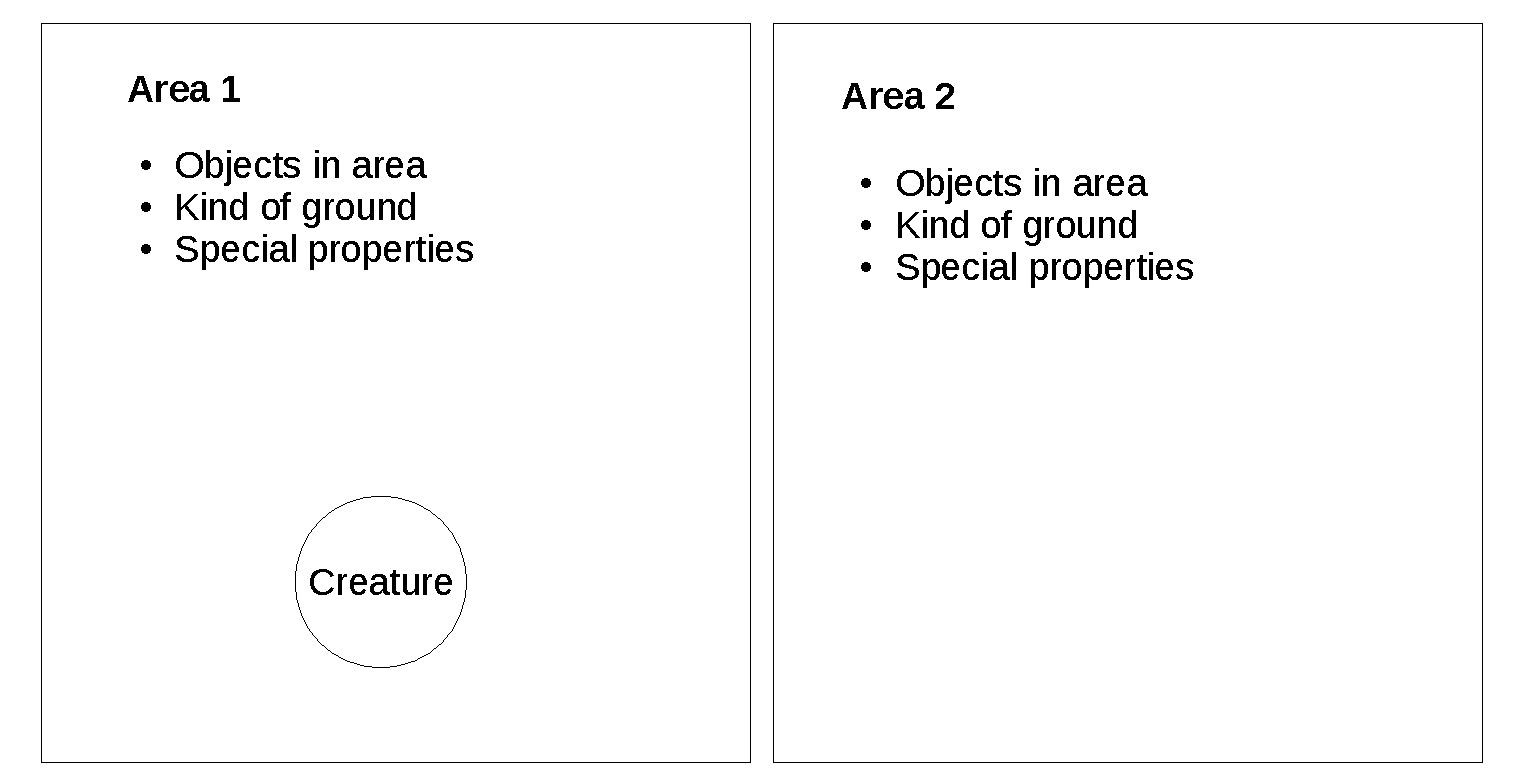
\includegraphics[scale=0.5]{combat0}

\subsection{Combat Areas}
In the diagram above we can see a basic schematic of a battle scenario, you can make these out of cardboard for your own games. It consists of two areas, here just called 1 and 2. Each area will obviously have a more descriptive name in an actual fight, and have actual properties detailed on it. The type of terrain should be noted so that players know how hard it is to move around the fight, and whether there are objects or circumstances they can take advantage of (like boulders they push down a hill, or a river they can knock enemies into). Creature tokens can be used to represent which players or enemies are currently in which area. Leaving a combat area that contains enemies results in a \textlf{Moment of weakness} (see Section~\ref{sec:aoo}).

\subsection{Distances and Radii}
A distance of 1 is size of 1 combat area (around 10 - 12 m in real life). In this system you measure a distance as the number of area boundaries crossed. So moving from one area to another is distance of 1. So to determine if an enemy is in range of a shooting attack you must count how many area borders the projectile must cross and compare it to the weapon range. A radius of 1 would cover a single area and ALL adjacent areas. An effect that is called \textlfirst{adjacent}, or radius 0, applies to a single combat area. 

\subsection{Basics of Movement}
Most creatures may transfer between combat areas, or move anywhere within one they are already in at the start of the turn, unless otherwise noted or modified by terrain. Movement actions cost 1 action point if the character wishes to change combat area. Normal movement in this manner is thus said to have a range of 1. 

\subsection{Basics of Attacks}
Attack-type actions represent making attempts to injure an enemy, they come in two varieties: ranged attacks, which are made with bows, guns, etc., and close-combat attacks which are made with swords, fists, etc. Successful attacks can batter the target, reducing its \textlf{endurance}. Once a creature's \textlf{endurance} depletes it is exhausted and further attacks can seriously injure it (this will detailed in the more advanced combat rules). A character can only make one attack per turn, unless otherwise modified. 

Declaring an attack costs 1 action point. During resolution the attacker and their target make an opposed check with \textlf{aim} and \textlf{deflect} respectively. If the attacker wins then the attack has struck home and moves on to roll damage checks.

\subsection{Close-Combat}
A character can make close-combat attacks against any creature within the same combat area as they are (range 0).

\subsection{Ranged}
A character armed with a ranged weapon can often attack enemies that are in different combat areas to itself. How far it is allowed to do so is defined by the weapon's range score. A range of 1 would allow shots to be fired at a target in any adjacent area to that of the firer. Draw a straight line between the shooter and target and count the number of area boundaries it passes over. 

\subsection{All-out attack}
The character channels all their energy into aggression. This attack action can be made with any weapon that has no \textlf{reload} rule, it costs 2 action points but grants \textlf{edge} on the damage roll (for one of the character's weapons if wielding two).


\section{Combat - More Details}

\subsection{Moment of Weakness}
\label{sec:aoo}
These are moments when an opponent opens their guard or shows vulnerability, allowing an attacker to strike unhindered. A creature subject to a \textlf{moment of weakness} suffers an immediate damage roll from one enemy within reach (radius 0 for human-sized creatures). Sometimes the enemy who may exploit the free hit is specified by the effect, otherwise the eligible enemy with the highest \textlf{cunning} gets the hit.
Each creature or player can make only one of this type of attack per round. 

\subsection{Resisting effects}
Some attacks/powers have special effects. These should always be potentially mitigated via a \textlfirst{resist} check. This involves an opposed roll between the \textlf{power} of the effect ($\dicenoprof$ or the user's \textlf{Might} if proficient) and the most appropriate choice from the victim's attributes. For instance, resisting poison might use \textlf{Resolve}, whereas avoiding being hypnotised would require \textlf{wit}.    

\subsection{Changing weapons}
To swap their current held the weapon a character must spend 1 action point.

\subsection{Other Types of Movement}
\subsubsection{Running}
A character can run, at a cost of 2 action points, they then add 1 to their movement range and gain an \textlf{edge} bonus on \textlf{deflect} checks for 1 round. 

\subsubsection{Retreat}
At a cost of two action points the character can make a normal move, while leaving an area occupied by enemies, and not suffer a \textlf{moment of weakness}.

\subsection{Armour}
Armour provides protection bonuses in the form of additional \textlf{Toughness}. A character's total is 8 plus armour bonuses. However, protection comes at a price and weighty armour makes certain tasks more difficult, like dodging, climbing, and swimming. 

\subsubsection{Light Armour}
This does not have adverse effects on the wearer as it is light and flexible. 

\subsubsection{Medium Armour}
\textlf{Medium Armour} applies an \textlf{edge} penalty to \textlf{Athletics} and \textlf{Stealth}.

\subsubsection{Heavy Armour}
\textlf{Heavy Armour} applies an \textlf{edge} penalty to \textlf{Athletics}, \textlf{Stealth}, and \textlf{Deflect}. Characters in \textlf{heavy armour} also have to spend an action point to get up if \textlf{knocked down} and suffer \textlf{edge} penalties on opposed attempts to get back up.

\subsection{Attacks that Hit}
If an attacker lands a successful attack on their foe, as described above, they may then make a damage roll to see if the blow injures the target. 

\subsubsection{Multiple Weapons}
If the character is using a weapon in each hand, they may attack with both for 1 action point. Only one opposed \textlf{deflect} vs \textlf{aim} check is made, but, each weapon gets separate damage rolls. Unless the character has the \textlf{Two-Weapon Fighting} \textlf{perk} (or other special rule) they suffer a \textlf{aim} \textlf{edge} penalty on such attacks.

\subsubsection{Damage Rolls}
\label{sec:dmg}
This represents whether or not a telling blow penetrates your target's armour.

A damage roll is a \textlf{power} check with the victim's \textlf{toughness} as \textlf{difficulty}. If the check succeeds then the victim loses \textlf{endurance} and, after reaching zero, collects wound effects (easily tracked of via cards) to monitor how much of a potentially lethal battering they have suffered. See Section~\ref{sec:wounding} for the effects of any damage inflicted in this way (or below for the basics).

\subsubsection{Basics of Damage}
If a character suffers a hit they lose \textlf{endurance} points. How many are lost depends on the \textlfirst{lethality} of the attack. The grades being normal, crushing, devastating, and vorpal. These remove 1,2,3, and 5 \textlf{endurance} points respectively. Once a character has no \textlf{endurance} left, further damage is accumulated as actual injuries which are tracked via \textlf{wound} effects. 

Against targets with zero \textlf{endurance}, an attack of normal lethality will just wound its victims (dealing a \textlf{wounded} effect), whereas crushing lethality inflicts the \textlf{badly-wounded} state, and \textlf{devastating} the \textlf{mortally wounded} effect. Vorpal attacks instantly slay their victim.
If a character is \textlf{wounded} they suffer an instance of the \textlf{Staggered} effect (an \textlf{edge} penalty to the next action). Very serious damage is referred to as \textlfirst{badly wounded}, which inflicts an \textlf{edge} penalty on all the victim's rolls. \textlfirst{Mortally wounded} characters will die if they do not receive medical attention and cannot make any strenuous actions. 


\subsection{Additional Attack Rules}
\label{sec:close-combat}
\subsubsection{Critical Hits}
For every $\dicecritlvl$ a damage roll exceeds the victim's \textlf{toughness} by, the \textlf{lethality} of the attack is upgraded by one level. This is to represent the effects of extremely telling blows.

\subsubsection{Penetrating Hits} 
If the target of an attack loses the opposed \textlf{aim}/\textlf{deflect} check by $\dicecritlvl$ or more then the attacker has achieved a \textlfirst{penetrating hit}, this allows associated damage rolls to gain one \textlf{edge} bonus per critical success threshold. 

\subsubsection{Ranged Weapons}
As with close-combat targets, the attacker and defender make a single opposed \textlf{aim}/\textlf{deflect} check. If the attack has multiple projectiles you simply make the appropriate number of damage rolls on a successful hit. These weapons are divided into two types.
First is shooting weapons: this subset encompasses bows, crossbows, and fire-arms. These weapons are operated to mechanically fire an arrow or similar projectile, requiring less exertion to use than it would to throw the projectile yourself. Shooting weapons suffer an \textlf{edge} penalty on \textlf{Aim} when used on targets within range 0.
Secondly, there are throwing weapons: this subset includes all types that are thrown by the force of a character's own arms/legs/limbs. 
All thrown weapons can be used effectively at point blank range (range 0). 





\section{Combat Areas - Terrain}
\label{sec:terrain}
\subsection{Open Terrain}
Grass, sand, tiles, gentle slopes or terrain that offers otherwise firm-footing is open terrain. This confers no bonuses or penalties to movement over it.

\subsection{Rough Terrain}
\label{sec:rough-t}
This includes: loose rocks, tree roots, rubble, tables and chairs, obstructions of about knee or waist height, and surfaces that are unstable/moving/irregular. Moving into or out of \textlf{rough terrain} costs 1 action point more than normal.

For characters riding or driving, moving in \textlf{rough terrain} requires a ride/drive check versus a \textlf{difficulty} (chosen by the GM) between 8 and 12 (depending on how rough the terrain is) to avoid being unseated or losing control. 

\subsection{Dangerous Terrain}
Marsh-land, fast-flowing water, quicksand, thin ice, brittle rock, pools of acid or hot mud; these sorts of things are \textlfirst{dangerous terrain}. Any character entering, occupying, or moving through this terrain takes a hit with \textlf{crushing lethality} that causes damage on a $\dicediffbase+$ regardless of \textlf{toughness}. \textlf{Rough terrain} movement restrictions apply here as well.

For characters riding or driving, \textlf{dangerous terrain} requires a riding/driving check versus a \textlf{difficulty} (chosen by the GM) between 11 and 16 to avoid being unseated.



\section{Combat Areas - Cover}
\label{sec:cover}
If a combat zone offers cover then any creature within the zone may claim a bonus to any deflect checks it makes. Cover is divided into three categories and examples will be given below.
\begin{table}[ht]
	\centering
	\caption{Cover Table}
	\label{tab:cover}
	\begin{tabular}{|l|l|l|}
		\hline
		Cover Type & Deflect Bonus & Hide Bonus\\ [0.5ex]
		\hline
		Soft & - & \textlf{edge}\\
		Medium & \textlf{edge} & \textlf{edge}\\
		Heavy & 2$\times$\textlf{edge} & \textlf{edge}\\
		\hline
	\end{tabular}
\end{table}

\subsection{Soft Cover}
Good examples of soft cover are: small trees, bushes, wooden crates, soft furnishings and other such items that provide little protection but may conceal you from your enemies, and so, grant an \textlf{edge} bonus on any rolls to hide in them. Objects that provide soft cover can be broken with a \textlf{might}/\textlf{power} check against \textlf{difficulty} 6-9.

\subsection{Medium Cover}
Sandbags, hedges, low walls, small rocks, solid furniture. These kind of things provide a moderate amount of protection and concealment from enemies and an \textlf{edge} bonus to rolls to hide in the cover. Objects that provide medium cover can be broken with a \textlf{might}/\textlf{power} check against \textlf{difficulty} 9-13.

\subsection{Heavy Cover}
Battlements, Large walls, trees, big rocks, barricades, serious furniture (made of stone or steel). These things are built to provide a lot of cover and protection and also grant an \textlf{edge} bonus to rolls to hide in the cover. Objects that provide heavy cover can be broken with a \textlf{might}/\textlf{power} check against \textlf{difficulty} 13-20.


\section{Combat Areas - Examples}

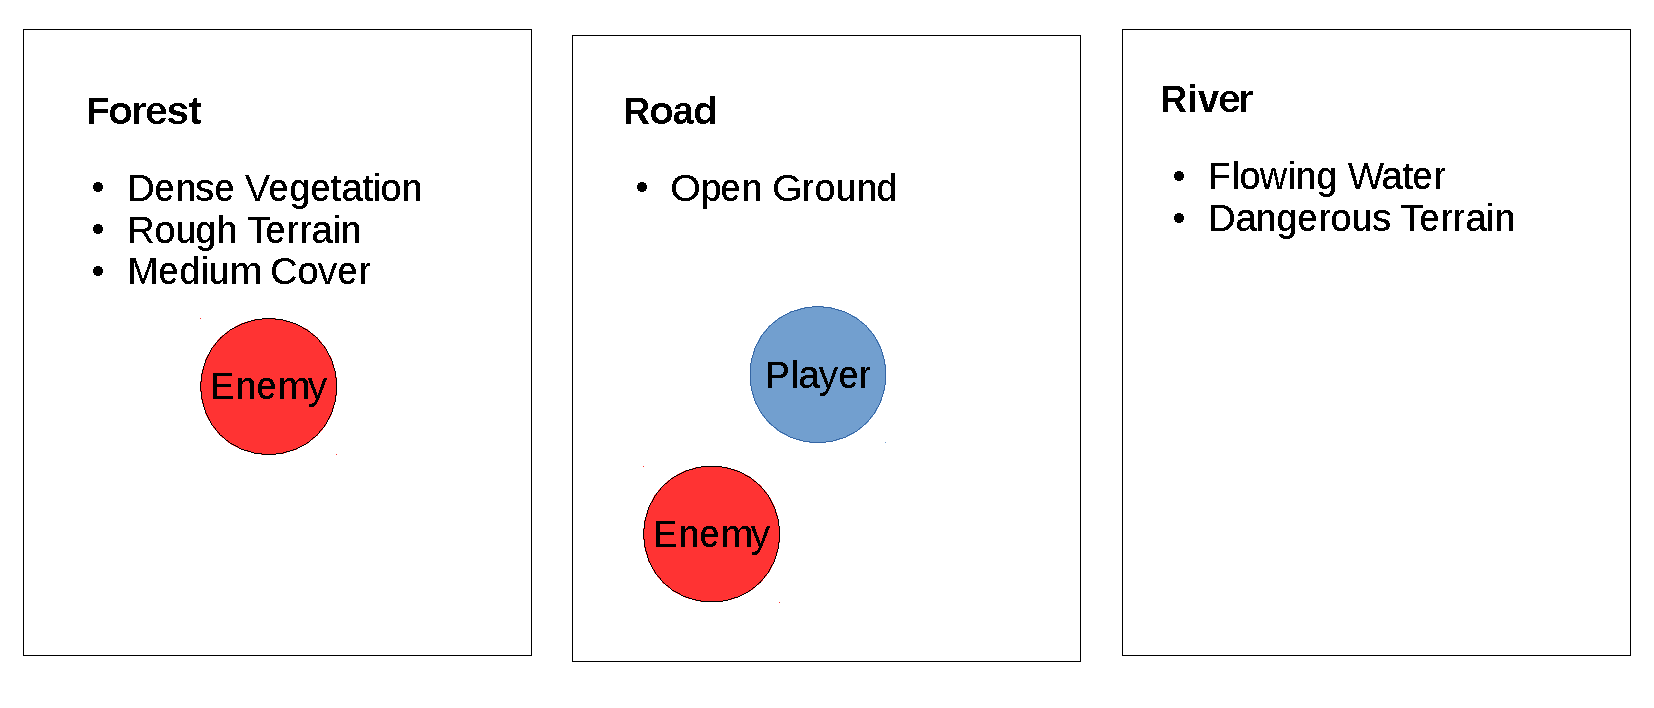
\includegraphics[scale=0.5]{combat1}


In our first example we see a fight with three combat areas. We can see it also has three participants, one player character and two enemies attacking them. The first area is the forest, which is \textlf{rough terrain} and provides medium cover. The road is open ground that confers no effects. Finally there is a river which is fast-flowing and thus \textlf{dangerous terrain}. We can see that in the road the player and enemy will be able to attack each other with any weapons. While the baddy hiding in the forest will be able to claim a cover bonus but will need a range 1 weapon to strike at the player.


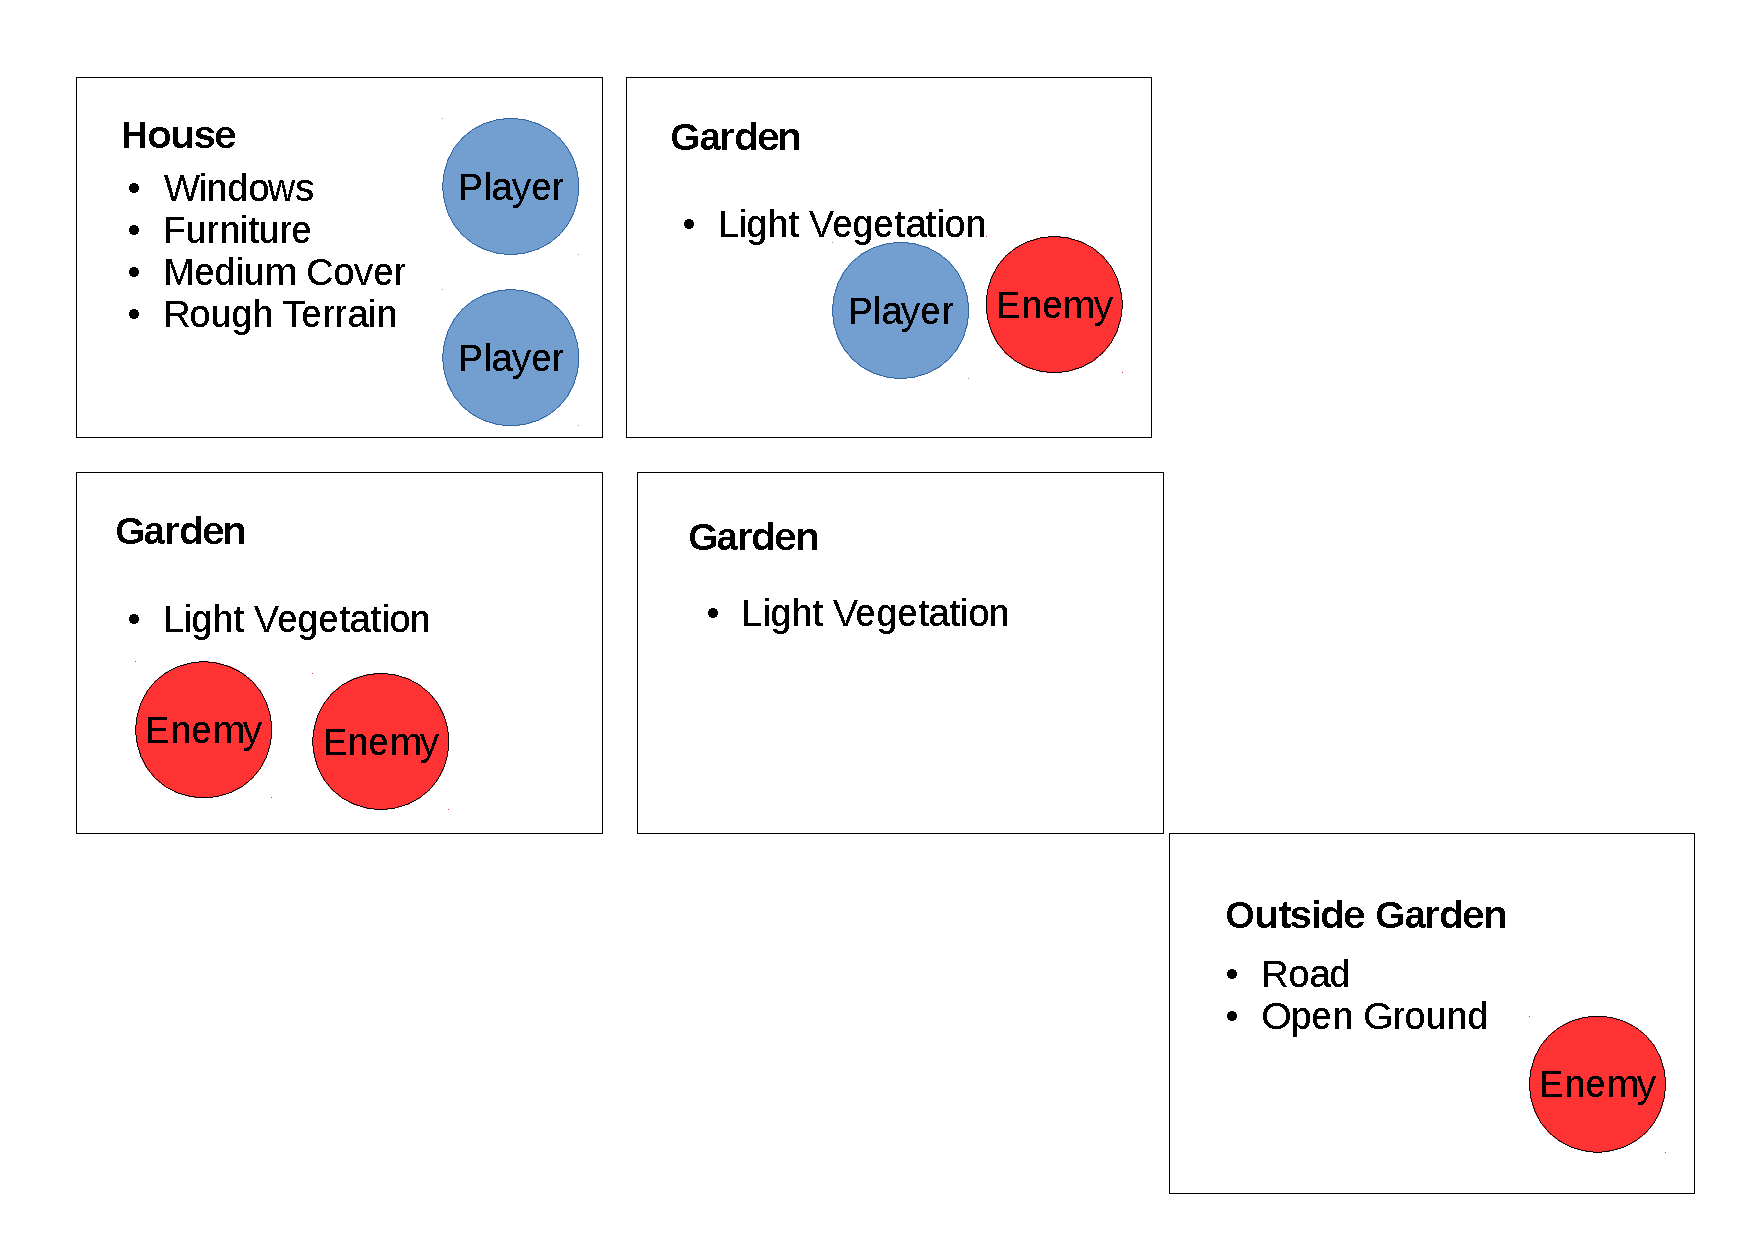
\includegraphics[scale=0.5]{combat2}

Our second example has a far more complex layout consisting of 5 areas. One is a house occupied by two player characters. The house provides medium cover to its occupants and they can attack out of the windows. Additionally, because it is a good defensive position it is labelled \textlf{rough terrain}, so enemies have difficulty moving into/through it. The garden has no special effect on combat and neither does the distant road. The players in the house will need range 1 weapons to hit the foes in the garden and range 2 to target the one out on the road. The player and enemy within one garden block can engage in either close-combat or fire ranged weapons at each other.



\section{Taking Damage and Wounding} 
\label{sec:wounding}
If a damage roll is successful against a creature then it either loses \textlf{endurance} or, when at zero, suffers a wound. How dangerous an attack is depends on the \textlf{lethality} of the weapon. Refer to Table~\ref{tab:lethal} and to the details in the sections below. If a character would be reduced to negative \textlf{endurance}, the lost points beyond zero are converted to wounds (i.e. -1 to \textlf{wounded} or -2 to \textlf{badly-wounded} etc).

\begin{table}[htbp]
	\centering
	\caption{Lethality Table}
	\label{tab:lethal}
	\begin{tabular}{|l|l|l|}
		\hline
		Lethality & Endurance loss & Wound \\
		\hline
		Normal & 1 & \textlf{Wounded} \\
		Crushing & 2 & \textlf{Badly wounded} \\
		Devastating & 3 & \textlf{Mortally Wounded} \\
		Vorpal & 5 & Instant death\\
		\hline
	\end{tabular}
\end{table} 

\subsection{Wounded}
Such a hit represents a flesh-wound and inflict an instance of the \textlf{staggered} effect on the victim (see \ref{sec:special}). The effect remains active until healed but the \textlf{staggered} only happens once.  

A character who receives two \textlf{wounded} effects replaces them with a \textlf{badly-wounded} effect.

\subsection{Badly Wounded}
If a character suffers a successful damage roll from a weapon with \textlf{crushing lethality} they are \textlf{badly-wounded}. They suffer an \textlf{edge} penalty on all rolls until remedied.

A man-sized character subject to two \textlf{badly-wounded} effects replaces them with \textlf{mortally wounded}.

\subsection{Mortally Wounded}
A \textlf{mortally-wounded} character cannot make actions and will die in three days unless they receive some medical attention. This status can only be removed by active healing. If a \textlf{mortally wounded} character is healed, change this effect to \textlf{badly wounded}.


\section{Recovery and Healing}
\textlf{endurance} is recovered completely if the character can rest for 8 hours. Otherwise, a short rest of around an hour restores 1 \textlf{endurance}.

A character that has suffered wounds can be healed via use of the Healing skill or by a non-player Healer. Without healing, a character heals one \textlf{wounded} effect every 3 days and one \textlf{badly-wounded} every 10 days.






\section{Special Actions and Situational Modifiers}
\label{sec:adv-spc}

\subsection{Anticipate}
A fighter can try and predict their opponent's next move. This costs 1 action point and requires an opposed \textlf{cunning} check. If you win then you can change your declared actions in response to the target. \textlf{critical Failure} means you suffer a \textlf{moment of weakness}.

\subsection{Light and darkness}
\label{sec:dark}
The lighting of an environment greatly influences the difficulty of fighting within it. There are three types of lighting: \textlfirst{full}, \textlfirst{low}, \textlfirst{dark}. \textlf{full} lighting has no effect, \textlf{low} incurs an \textlf{edge} penalty on \textlf{aim}, and \textlf{dark} means the character cannot see at all outside of 6 m (1 combat area) and also incurs \textlf{low} light penalties.

\subsection{Sneak Attacks}
\label{sec:sneak-attk}
A target that does not know of your presence, aggressive intent, or is otherwise fully engaged in combat with someone else (the target must have been unaware of your combat participation, if not your presence) is vulnerable to \textlfirst{sneak attacks}.

The victim of a \textlf{sneak attack} gets no opportunity to \textlf{deflect}, unless otherwise modified.
Such attacks always gain an \textlf{edge} bonus to damage rolls. Additionally, they have \textlf{heavy weapon} 1 when made with \textlf{small} weapons, such as daggers, or with specialist tools, such as garrotte wire. Multiple \textlf{perks} can improve \textlf{sneak attacks}. \textlf{Small} weapon bonuses are lost on \textlf{Huge}, or larger, targets.

\subsection{Feints}
\label{sec:feint}
A feint costs one action point and requires an opposed cunning check with the target. Success allows you an \textlf{edge} bonus to \textlf{aim} this round, while \textlf{critical failure} results in a \textlf{moment of weakness} that can be exploited by the victim only. This has no effect with ranged weapons unless otherwise modified.

\subsection{Bull-rush}
\label{sec:bull}
This represents the character attempting to plough through enemies, knocking them down in the process. This costs 2 action points and is resolved as an opposed might check. The heavier participant gets an \textlf{edge} bonus on this check. If a character moved this turn they also gain an \textlf{edge} bonus. This action may have up to two adjacent targets. 

If the character using the \textlf{bull-rush} move wins, the target is knocked to ground. If the defender scores higher than the bull-rushing character, they are stopped in their tracks and suffer a \textlf{moment of weakness} exploitable by the target.

\subsection{Unarmed Attacks}
A character can attack their opponents with fists and feet, or other appendages. Unarmed characters may make a single punch/kick for 1 action point, this fighting style has its own weapon proficiency.

\subsection{Trip}
Attempt to entangle your foe's legs with your weapon's haft, or pointy bit built for tripping. This modifies an attack action: replace a damage roll with an opposed \textlf{cunning} check, should you win the target is \textlf{knocked down} (see Section~\ref{sec:special}). Weapons with the \textlf{Trip} rule do not need to sacrifice a damage roll.

\subsection{Disarm}
Even the mightiest warrior can be flummoxed by the loss of their precious sword.
This modifies an attack action: replace a damage roll with an opposed \textlf{wit} check, should you win the target cannot use their current weapon without spending 1 action point to retrieve it and suffering a \textlf{moment of weakness}. Weapons with the \textlf{disarm} rule do not need to sacrifice a damage roll.

\subsection{Grapple}
You can attempt to wrestle your foe into an immobile state at the cost of 1 action point. Provided you have at least one free hand, you make an opposed \textlf{Might} check with your target. If you win, the target is now \textlf{grappled}. However, if you score a \textlf{critical failure}, you suffer a \textlf{moment of weakness} that can be exploited by the target. A \textlf{critical success} makes your target lose 1 action point. It costs 1 action point each round after the first to maintain a grapple.

\textlf{Grappled} foes cannot make any movement actions until they break free of the \textlf{grapple}, this costs 1 action point and requires that they win an opposed \textlf{Might} check with the grappler. If they are forced to move by some external effect then the grapple breaks automatically.

\subsection{Shove}
This costs 1 action point and involves an opposed \textlf{Might} check with the target. If the shover is successful the target is either knocked down or moved into an adjacent combat area (at the shover's discretion). \textlf{critical failure} results in shoving character experiencing a \textlf{Moment of weakness}. \textlf{critical success} results in the victim suffering a damage roll.

\subsection{Defensive stance}
This costs 1 action point. The character gains an \textlf{edge} bonus to \textlf{deflect} the next attack.

\subsection{Prepared Actions}
\label{sec:prep}
A \textlfirst{prepared action} is one that the character does not wish to make immediately. Instead, they specify the actions they wish to make, as for a normal turn, but, in addition, must specify a condition for the activation of the prepared actions. Such as: they will make their actions in response to a specific action made by an enemy, or to an environmental event, like a wall collapsing. Having specified their prepared actions, the character then waits and executes the prepared action when the condition is met. If the condition is not met by beginning of the next action declaration, then the prepared action is not performed and the fighter may act as normal.

\subsection{Rage}
Many cultures hold that great warriors are capable of being consumed by a battle rage, indeed in the heat of battle, with adrenaline pounding through your veins, it is easy to simply let your instincts loose and lapse into a raging frenzy. In such a condition a warrior is legendarily hard to stop, they can suffer wounds that would kill a normal man and still continue to fight with unbridled savagery. However, this rage makes them reckless, as heedless of danger or injury they hurl themselves into enemies, bringing death and destruction with them.

The mechanics below detail how this berserker fury affects characters and how they can initiate such a state.  

\subsubsection{Becoming Enraged}
A character becomes \textlfirst{enraged} if under extreme emotional strain while fighting, although particularly volatile personalities may become \textlf{enraged} more easily. Otherwise a character with the Berserker \textlf{power} can trigger an \textlf{enraged} state once per day.

\subsubsection{When Enraged}
An enraged character seeks to enter close combat with the nearest enemy at all times and cannot take prisoners, they go only for the kill. If wielding a firearm-type weapon, they may fire it at range (while moving as required). Enraged characters have an \textlf{edge} penalty on \textlf{deflect} checks and but an \textlf{edge} bonus on damage rolls.

Rage drains one point of \textlf{endurance} each round and ends when the character has no points left. A character cannot \textlf{enrage} unless they have at least one point of \textlf{endurance}. The first time the character causes damage during a round they regain 1 \textlf{endurance}.








\section{Enemies and Monsters}
\label{sec:monsters}
Enemies come in several categories, ranked according to their defining characteristics.

\subsection{Mundane Enemies}
These are generally creatures of humanoid or smaller size, this category is largely composed of humanoid soldiers, wolves or similar beasts.
\subsubsection{Abilities and Attributes}
Mundane enemies have no \textlf{heroism/villainy}, they can have \textlf{aim} bonuses ranging from 0-2, 0 being an inexperienced impromptu fighter and 2 being a well trained soldier. Such foes are likely to have zeros for most attributes, although the more experienced combatants may be suitably tougher and stronger (no attributes above 1 however). 
\subsubsection{Tactics}
These enemies are followers, they need to be lead. Without a leader to direct them, they are likely to be easily demoralised by powerful opponents or to simply attack the enemy they feel is the most threatening. Such behaviour is over-ridden in the presence of a leader. Mundane enemies suffer the \textlf{panic} effect (see section~\ref{sec:special}) if they run out of \textlf{endurance} or if they suffer a \textlf{badly-wounded} effect. Enemies who believe in their cause, or are mindless, are immune to this. When being lead, a mundane creature may use its leader's leadership score to make courage checks.

\subsection{Elite Enemies}
These are generally creatures who are extremely proficient combatants or are enhanced by some magical or technological power.
\subsubsection{Abilities and Attributes}
Such fighters are likely to have above average attributes, e.g. between one and three at levels 1 or 2. Elite enemies do not have any heroic attributes but may have multiple combat proficiencies.
\subsubsection{Tactics}
Such enemies are independent, they do not need to be lead, but are more effective with a leader to direct them. These foes are unlikely to be easily demoralised or intimidated by powerful opposition and will coordinate and work together to defeat stronger opponents. suffer the \textlf{panic} effect (see section~\ref{sec:special}) if they run out of \textlf{endurance} or if they suffer a \textlf{badly-wounded} effect. Enemies who believe in their cause, or are \textlf{mindless}, are immune to this. When being lead, an elite creature may use its leader's leadership score to make courage checks.

\subsection{Enemy Leaders}
These are generally creatures who are proficient combatants but are also skilled at directing the actions of underlings.
\subsubsection{Abilities and Attributes}
Leader enemies are similar to elites in attributes but also have leadership proficiency.
\subsubsection{Tactics}
Such enemies co-ordinate their allies, using their leadership skill to enhance their fighting prowess and allowing lesser allies to adopt more sophisticated tactics. Leaders will attempt to avoid combat unless they are heavily reinforced. In other regards they behave similarly to elite enemies.

\subsection{Heroic Enemies}
These enemies are powerful heroes, much like the player-characters, except that they oppose the heroes for whatever reason that the GM decides should motivate them.
\subsubsection{Abilities and Attributes}
These enemies are individually as capable and powerful as player characters, sometimes more-so, and thus follow the same rules for heroic attributes and determining combat statistic scores. Heroic foes have attributes generated in a similar manner to players, although the Game Master may decide to give them more, or less, points to spend.
\subsubsection{Tactics}
Such enemies are leaders, they direct lesser foes in ways that will maximise their own advantage within a fight, they will also use their heroic attributes to the maximum possible effect. The presence of such enemies inspires and emboldens lesser enemies, making them less susceptible to intimidation and fear. Heroic enemies may surrender if they are severely injured or near death.

\subsection{Monsters}
These are enemies that are usually at least large creatures and often huge or titanic creatures (see Section~\ref{sec:special}). However, enemies that possess incredible supernatural powers or extreme natural abilities might fall into this field as well.
\subsubsection{Abilities and Attributes}
Such creatures have access to unique abilities or methods of fighting that might not need to depend on heroic attributes, monsters generally have low \textlf{aim} bonuses, as many monsters are large and have trouble making rapid manoeuvres. However, they have immense strength and aggression, larger creatures having high \textlf{power} to represent this. They may also, simultaneously, possess heroic attributes, but this is not needed, they are quite often mighty enough as it is. 
\subsubsection{Tactics}
These enemies are hugely dangerous and will simply exploit the powers, size or strengths that make them monsters in order to win. They attack enemies that seem the easiest prey, or those that otherwise attract their attention, unless they have the opportunity to get more than one foe at once. Some monsters may be extremely stupid, this limited intelligence can be exploited by players to distract or confuse such foes, such monsters may need a handler to direct them and counter-act their innate lack of quick wits. Monsters do not know the meaning of surrender or fear.


\section{Unnecessarily Advanced Combat Rules}

\subsection{Mounted Combat}
\label{sec:mountandblade}
Mounted combat is, as is quite obvious, combat while riding upon a mount. While mounted you gain the advantage of speed, mobility and the ability to trample your foes in addition to the devastating effects of a mounted charge.

\subsubsection{Mounted Charge}
Certain weapons, such as the lance and horse sword, utilise the power and speed of a mounted charge to the full, inflicting great damage as they smash into the hapless foe. This action costs 2 action points and allows a normal movement and attack action. The \textlf{difficulty} of the required ride check is 11 + 1 for rough and + 2 for \textlf{dangerous terrain} (with a possible dismount on failure). 

A mounted charge grants the rider an \textlf{edge} bonus to damage rolls this round.

\subsubsection{Trample}
You may attempt, while charging, to ride your opponent down and trample over them. This trample attempt requires a check opposing the mount's \textlf{aim} and victim's \textlf{deflect}. If the target wins they evade the trample, and you suffer a \textlf{moment of weakness} that the intended victim may exploit. However, if the \textlf{deflect} fails, the target is trampled beneath your mount's hooves/feet/wheels/appendages of motion. This results in the victim being knocked down and taking three hits which have \textlf{power} equal to that of the mount with an \textlf{edge} bonus. You cannot trample a target that is larger than you and your mount.



\section{Universal Special Rules}
\label{sec:special}
This is a collection of special rules that apply in all campaign settings and always mean the same thing regardless of context.


\subsection{Conditions}
These are negative statuses that a character can become subject to. 

\subsubsection{Vulnerable}
A powerful blow can sometimes open up a fighter to being easily finished off. All attacks directed at the victim benefit from an \textlf{edge} bonus to damage rolls for the effect's duration (default is 1 round).

\subsubsection{Staggered}
The shock of injury is a difficult thing to ignore and can incapacitate even the most hardened fighters. A \textlf{staggered} creature makes its next roll with an \textlf{edge} penalty. A character who has been subjected to X such effects faces the penalty on the next X rolls. 

\subsubsection{Knocked Down}
A creature that is \textlfirst{knocked down} loses its footing and falls over. Such a creature is \textlf{vulnerable} until it can stand up. Standing up can be done only in your own turn. It costs no action points if the character wins an opposed \textlf{might} check with all adjacent opponents, otherwise it costs 1 action point.

\subsubsection{Blind}
A \textlfirst{blinded} creature has an \textlf{edge} penalty on both \textlf{aim} and \textlf{deflect} for the effect's duration. In addition, it must randomise direction if it wishes to move.  

\subsubsection{Immobilised}
An \textlfirst{immobilised} creature cannot move, either due to some magical malaise or due to having suffered damage to its legs.

\subsubsection{Crippled}
The sudden shock of a well-placed blow can often neuter retaliation. If a \textlfirst{crippled} creature attempts to make attacks in its next turn these cost 1 more action point than normal. 

\subsubsection{Cursed}
A \textlfirst{cursed} creature is afflicted by a malignant magical effect sapping its luck and increasing the chance of misfortune. \textlf{Critical success} rolls made by a \textlf{cursed} creature are treated as \textlf{critical failures}. \textlf{Curse} lasts until removed.

\subsubsection{Bleeding}
This state represents severe bleeding. It lasts 2 rounds, each round the victim must make an opposed check: their \textlf{resolve} against your \textlf{might}. Their failure results in the loss of 1 \textlf{endurance}. 

\subsubsection{Fear}
If a character is afflicted by this effect they must make a \textlf{resolve} check against a difficulty, chosen by the GM, based on how scary the situation is. Should the character fail, they suffer an \textlf{edge} penalty on \textlf{aim} checks, each subsequent turn the character may try to pass the check again. 

\subsubsection{Terror}
If a character is afflicted by this effect they must make a \textlf{resolve} check against a difficulty, chosen by the GM, based on how scary the situation is. Should the character fail, they must spend each turn cowering in fear. Each subsequent turn the character may try to pass the check again.

\subsubsection{Panic}
A non-hero creature may \textlfirst{panic} if it suffers considerable injury. If an elite or mundane enemy runs out of \textlf{endurance}, or is \textlf{badly-wounded}, it must make a \textlf{resolve} check vs \textlf{difficulty} 13. Should it fail, it flees or surrenders. In general, intelligent creatures will surrender, but this is up to the Game Master's choice. Note that the presence of a commander or leader will prevent weaker creature from giving up so easily. In this case the creature may use it's leader's leadership score for panic-related checks.

\subsubsection{Poisoned}
Poisoned is a state that results from harmful chemicals being introduced into the victim's system. A poisoned attack that injures a creature, poisons that creature if it fails a \textlf{resolve} check versus a \textlf{difficulty} associated with the virulence of the poison and the size of the dose. A \textlf{poisoned} character has one fewer action point in combat (to a minimum of 1) until cured of the poison.


\subsection{Additional Weapon Effects}

\subsubsection{Cumbersome}
Weapons with this rule are either massively heavy or just awkward to manoeuvre. They cost an extra action point to make attacks with.

\subsubsection{Reach}
\textlfirst{Reach} represents the ability of close-combat weapons, like spears, to attack from a longer distance. A character with a \textlf{reach} weapon can make a free attack action each turn against a single enemy that enters their combat area, provided they are in \textlf{defensive stance}.

\subsubsection{Rending}
A well-placed blow from a \textlfirst{rending} weapon rips deep into the target. \textlf{Penetrating} hits from \textlf{rending} weapons benefit from a \textlf{lethality} upgrade.

\subsubsection{Massive Damage}
A weapon with \textlfirst{massive damage} does exactly as their name suggests. Thus, they have an \textlf{edge} bonus on their damage rolls, making mayhem all the more likely. 

\subsubsection{Heavy Weapon X}
(X is an integer) A \textlf{heavy weapon} scythes through mortal flesh and bone with supreme ease, laying waste to all but the hardiest of creatures. Upon succeeding on a damage roll with such a weapon, the wielder may repeat the roll. These repeat rolls stop after X extra rolls or when a roll fails. Each time they succeeded on the extra rolls the \textlf{lethality} of the attack is upgraded. \textlf{critical success} on these rolls means a double \textlf{lethality} upgrade.

\subsubsection{Burst X}
(X is an integer) \textlfirst{Burst} represents attacks that explode, spray, splash, or carve into a wide area of flesh. An attack with \textlf{burst} X causes 1 + X damage rolls on a successful hit, rather than just one. 

\subsubsection{Penetration X}
(X is an integer) A weapon with \textlfirst{penetration} is designed to deal with heavily armoured opponents, sliding into weak-points or just inflicting blunt trauma through armour. Attacks from this weapon count the target's \textlf{toughness} as reduced by X, but cannot reduce it below $11$ in this way.

\subsubsection{Cleave X}
(X is an integer) An attack with \textlfirst{cleave} is one that can sweep in great arcs, cutting through many hapless foes with each swing. Such an attack may target up to X enemies at once. The attacker rolls once with their \textlf{aim} and each defender rolls with their \textlf{deflect}.

\subsection{Additional armour effects}

\subsubsection{Bulwark}
Heavy plates of steel turn all but the most determined blows. Armour with this rule negates the bonuses conferred by the \textlf{Penetration} rule on incoming attacks.

\subsubsection{Adamant}
Some armour is so thick and heavy that it is almost impervious, even to weapons that shear through other protective gear. This grants immunity to \textlf{Rending} effects.



\subsection{Creature-Type Rules}

\subsubsection{Large Creature}
A creature is declared \textlf{large} if it exceeds 3 m in the main dimension (height, length,width depending on creature geometry). Thus, such creatures can only hide in medium or better cover but gain \textlf{cleave} 2 on all close-combat attacks. A \textlf{large} creature has an innate bonus of +1 \textlf{power}. Such a creature has 2 extra \textlf{endurance} points.

\subsubsection{Huge Creature}
Such vast beasts barely notice the damage inflicted by even the largest weapons a man can wield. In consequence they have 4 extra \textlf{endurance} points. Their colossal might means that these creatures also have \textlf{cleave} 3 on all close-combat attacks. \textlf{Huge} creatures have an innate bonus of +2 \textlf{power} and the size threshold to be declared \textlf{huge} is a requirement of least 6 m in the main dimension (height, length, or width depending on monster geometry). 

\subsubsection{Titanic Creature}
These behemoths are all but inured to the attacks of normal weaponry. In consequence they have 6 extra \textlf{endurance} points. \textlf{Titanic} creatures have \textlf{cleave} 4 on all close-combat attacks and \textlf{massive damage} against smaller targets. \textlf{Titanic} creatures have an innate bonus of +3 \textlf{power} and the size threshold to be declared \textlf{titanic} is a requirement of least 12 m in the main dimension (height, length, or width depending on monster geometry). Such beasts have range 1 on their close-combat attacks. 

\subsubsection{Small Creature}
Diminutive creatures are easily missed, even by the most vigilant of larger things. Consequently they get + 1 \textlf{deflect}.

\subsubsection{Mindless}
\textlfirst{Mindless} creatures have no thoughts, emotions, fear or creativity. Because of this, \textlf{mindless} creatures are immune to many occult powers, as well as the \textlf{fear}, \textlf{terror}, and \textlf{panic} effects. These creatures cannot use any advanced combat rules (no \textlf{flanking}, \textlf{sneak attacks} etc) apart from \textlf{grapple} and \textlf{bull-rush}. Mindless creatures are considered destroyed when they run out of \textlf{endurance}.



\subsection{Weapons and Special Attacks}

\subsection{Throw}
Weapons with the \textlf{Throw} rule are finely balanced for use as projectiles. Thus, weapons without this rule confer an \textlf{edge} penalty to \textlf{Aim} when thrown. 

\subsubsection{Dual-Wielding}
A character can wield a weapon in each hand if they so desire. While employing such an armament the fighter makes only one \textlf{aim} roll, but a separate damage roll with each weapon if their attack hits. For weapons with \textlf{reload} rules, reloading takes 1 action point longer but both weapons are reloaded together. 

All characters dual-wielding have an \textlf{edge} penalty to \textlf{aim} without the \textlf{Two-Weapon Fighting proficiency}.

\subsubsection{Small}
\textlfirst{Small} weapons represent dagger-sized implements. These can used with great speed and easily concealed but tend to lack reach. Thus, they incur an \textlf{edge} penalty to close-combat \textlf{aim}. This penalty is negated against \textlf{Vulnerable} targets, during \textlf{sneak attacks}, when paired with a larger weapon, or via the \textlf{close quarters perk}.






\chapter{Perks}
\label{chap:perks}
These are skills and talents learned or gained by a hero through the course of their adventures. They can be purchased through the expenditure of experience points with their cost given in brackets. Note that upgrades change their parent \textlf{perk}, they do not occupy a new \textlf{perk} slot.

\section{General proficiencies}
These do \textbf{not} occupy equipment slots for passive or active \textlf{perks}, their effect is always active.

\subsection{Close quarters (2)}
Up-close and personal. The character is an expert at very close range engagements with \textlf{small} weapons. This negates close-combat penalties associated with such weapons.

\subsection{Hero/Villain (0)}
(Requires \textlf{Reputation} level 5) The character has become famous, their praise is much sung, or vile deeds whispered of, in local taverns. The character may increase one \textlf{natural attribute} by 1 point.

\subsection{Instrument Proficiency: X (2)}
(Where X is a musical instrument type) The character has learned to play a chosen type of musical instrument (X) and no longer suffers the unknown-instrument penalties when playing this type of instrument.  

\subsection{Language: X (2)}
(X is a language) The character has complete fluency in the chosen language. 

\subsection{Skill proficiency: X (3)}
(Where X is a skill) The character is proficient with skill X, see Section~\ref{sec:skill-prof} for details.

\subsection{Master: X (5)}
(Requires \textlf{Skill proficiency: X}) The character has achieved mastery of their art. Any check for the mastered skill X an \textlf{edge} bonus.

\subsection{Two-Weapon Fighting (3)}
This allows the character to fight with two weapons simultaneously without an \textlf{edge} penalty on \textlf{aim} checks.

\subsection{Weapon proficiency: X (2)}
The character is proficient in the class of weapons X. Classes should be chosen on similarity of use, e.g. for a medieval setting: swords, bows, daggers, blunt, axes, crossbows, firearms, and pole-arms. One type that is always available is unarmed.


\section{Active perks}
These open up new actions that a character can make and they must occupy an equipment slot for active \textlf{perks} to be usable.
\label{sec:active}

\subsection{Acrobatic Attack (4)}
(Requires \textlf{Acrobatic movement}). This costs 1 action point and allows the character to make both an \textlf{acrobatic movement} and attack action (against a target within range during the movement).


\subsection{Aimed shot (4)}
This costs two action points and allows the character to make a single ranged attack with an \textlf{edge} bonus on \textlf{Aim} and associated damage rolls.


\subsection{Berserker (4)}
You mad, bro? The character has harnessed their inner rage. This allows them to voluntarily \textlf{enrage} once per day.

\subsubsection{Upgrade: Berserkergang (2)}
(Requires \textlf{berserker}) The character has mastered their inner fury allowing them to \textlf{Enrage} twice per day.

\subsubsection{Upgrade: Endless rage (3)}
(Requires \textlf{berserker}) Becoming \textlf{enraged} restores the character's \textlf{endurance} to its maximum value. Additionally, the character can still become \textlf{enraged} when they have no \textlf{endurance} left.

\subsubsection{Upgrade: Seething rage (2)}
(Requires \textlf{berserker}) The character's rage is turns them into a  highly focussed killer. This grants the \textlf{enraged} character an \textlf{edge} bonus to \textlf{aim}, but a similar penalty to \textlf{deflect}.


\subsection{Blind Side (4)}
A deft feint allows the character enough room to fire their ranged weapons against close-combat assailants. When using a ranged weapon against a target within range 0 you may feint as though you were using a close-combat weapon. Success on the \textlf{feint} means you additionally ignore the normal \textlf{edge} penalty on shooting weapon hit rolls for targets within range 0.


\subsection{Butcher's blow (3)}
The force of the character's strikes cause them to inflict horrendous damage. This can declared when declaring an attack, the cost is increased by 1 action point. Should the attack cause damage, the target is subject to the \textlf{cripple} effect. This effect applies only to creatures a maximum of 1 size category larger than the character.


\subsection{Deeds Not Words (4)}
(Requires \textlf{Skill proficiency: leadership}) Any time the character defeats a foe in combat the character may make a leadership action, that would otherwise cost 1 action point, for free. Defeat is defined by the enemy fleeing, surrendering, being incapacitated, or dying.


\subsection{Desperate Mechanisms (3)}
The character may reduce the \textlf{reload} action point costs of ranged weapons by 1. If they do so, they experiences an \textlf{edge} penalty on \textlf{aim} for their next attack.


\subsection{Diplomat (3)}
The character has great skill in pacifying angry or confrontational speakers, allowing them to do so with an opposed \textlf{resolve} check.


\subsection{Dragon Kick (2)}
(Requires \textlf{Weapon proficiency: unarmed}) The character may make an unarmed attack, after moving, in the form of a flying kick. This allows them to bypass intervening obstacles, and any such attacks that succeed on their damage roll also knock the target down. The knock down effect applies only to creatures a maximum of 1 size category larger than the character.


\subsection{Extra Sneaky (5)}
At a cost of 1 action point, the character's \textlf{sneak attacks} damage rolls gain a bonus level of \textlf{critical success} this turn.


\subsection{Flurry of Blows (3)}
A risky manoeuvre, the fighter replaces a considered attack with a hail of furious strikes. The character may declare they are making a flurry attack, in which case they may make an extra damage roll with a successful hit. However, the character suffers an \textlf{edge} penalty to \textlf{aim}. This cannot be used if the weapon requires \textlf{reload} actions.

\subsubsection{Upgrade: Barrage (3)}
(Requires \textlf{Flurry of Blows}) The character may use the \textlf{Flurry of Blows} effect twice, the second use incurs an \textlf{edge} penalty to \textlf{deflect} instead. 


\subsection{Frothing fury (4)}
(Requires \textlf{berserker}) While \textlf{enraged} the character may spend 2 action points to make an \textlf{all-out attack} against all adjacent enemies. Additionally, this costs 1 \textlf{endurance} point.


\subsection{Guard breaker (3)}
This attack knocks the foe off balance. The character may declare this special attack for 1 action point. This inflicts no damage roll, instead make an opposed roll with your \textlf{might} versus the target's \textlf{resolve}. If you win, the target suffers an \textlf{edge} penalty on \textlf{deflect} and becomes \textlf{vulnerable} to the next attack action directed against it. 


\subsection{Iron Hand (3)}
The character's blows are capable of tossing enemies aside like a child's toys. This is a special attack action that costs of 2 action points. If the attack hits, it inflicts no damage. Instead, the target is knocked flying, up to a distance of range 1 in a chosen direction, while also being subject to a \textlf{knocked-down} state. The victim suffers no damage unless they collide with an obstacle (i.e. enters \textlf{rough terrain} or cover). This effect applies only to creatures a maximum of 1 size category larger than the character.

\subsubsection{Upgrade: Fist of Steel (3)} 
(Requires \textlf{Iron-Hand}) As long as the character is unarmed, \textlf{Iron-Hand} attacks inflict damage in the same manner as normal unarmed attacks, in addition to their special effects.


\subsection{Kick `em while they're down (5)}
At a cost of 1 action point, damaging \textlf{sneak attacks} made in this turn cause the victim to be afflicted with the \textlf{vulnerable} status.


\subsection{Lightning Fast (4)}
The character reacts so quickly that, during action declaration in combat, they may seize the initiative for their side at a cost of 1 action point. A character may not use \textlf{Lightning Fast} more than once per encounter (additionally, each side in combat can only benefit from this once per encounter).

\subsubsection{Upgrade: Swift as Death (2)}
(Requires \textlf{Lightning Fast}) The character has an \textlf{edge} bonus on \textlf{aim} and \textlf{power} checks during a turn when they have triggered \textlf{Lightning fast}.


\subsection{Martial Skill (3)}
At a cost of 1 action point the character's attacks this turn, with any close-combat weapon, count as having the \textlf{trip} and \textlf{disarm} rules. 


\subsection{Meteor Strike (2)}
(Requires \textlf{Weapon proficiency: unarmed}) The character gathers all their strength and makes a single unarmed attack, with only a single damage roll, this round. If they do so, this attack makes its victim \textlf{vulnerable} to the next damage roll it suffers.


\subsection{Now you see me, now you don't (5)} 
(Requires \textlf{Skill proficiency: stealth}) The character may attempt to use the \textlf{stealth} skill while in combat for 1 action point, fading seamlessly into the background. Additionally all attacks made after hiding are \textlf{sneak attacks} but reveal the presence of the character. While hidden, the character only incurs \textlf{moment of weakness} penalties if the potential attacker detects them.


\subsection{On the Hunt (4)}
The character zeros-in on their prey. The character may select a target against which they gain \textlf{edge} on aim and \textlf{deflect}. However, they suffer a similar penalty against all other targets. A new target may only be nominated once the present target is dead, defeated, or hostilities cease.


\subsection{Pistol Whip (4)}
When using a ranged weapon that can be wielded in one hand the character may make a ``Pistol Whip'' in place of a \textlf{sneak attack}. This is a close-combat attack that knocks the target down if it succeeds in causing a wound, if the victim fails \textlf{resolve} versus the \textlf{power} of the attack they are also rendered unconscious. This effect applies only to creatures a maximum of 1 size category larger than the character.


\subsection{Plan B (3)}
(Requires \textlf{Duelist}) Whenever one of the character's attacks is \textlf{deflected}, while in \textlf{Duelist} mode, they may make a free action drawing and throwing/firing a \textlf{small} weapon (this doesn't provoke a \textlf{moment of weakness} or suffer penalties for close range).


\subsection{Power attack (3)}
Enemy not dying? Just hit it harder! The character can declare a close-combat attack as a ``power attack''. This makes it cost 1 extra action point but grants + 1 \textlf{power} on damage rolls. 

\subsubsection{Upgrade: Thews and sinews (2)}
(Requires \textlf{Power attack}) \textlf{Power Attack} also upgrades the \textlf{lethality} of associated damage rolls. However, the character suffers an \textlf{edge} penalty on \textlf{aim} for such attacks.


\subsection{Reckless strike (3)}
The character can declare a close-combat attack to be a ``reckless strike''. Such an attack has an \textlf{edge} bonus to \textlf{aim} but the character incurs and \textlf{edge} penalty on \textlf{deflect} for one round.


\subsection{Splatter (3)}
The violence of your blows causes the blood of your foes to stain the soil. This can be used when declaring an attack, the cost is increased by 1 action point. Should the attack cause damage, the target is subject to the \textlf{bleeding} effect.


\subsection{Suppressing fire! (4)}
The character fires an indiscriminate volley of projectiles, forcing enemies and allies alike to get their heads down. This costs one action point, the character targets an area of radius 0, moving into, through, or out of the target area costs 1 extra action point for 1 round. This attack cannot be made with a weapon that requires action points be spent to reload it between shots.


\subsection{The ol' one-two (3)}
A close quarters manoeuvre where a quick punch is used to make room for firing a ranged weapon. This special attack costs 2 action points. Make an unarmed attack, if it hits you may perform damage rolls for both the unarmed hit and for a shooting-type, ranged weapon you are wielding. Note that it must be fireable with one hand (so no bows, but cross-bows or firearms are fine). 


\subsection{True Grit (3)}
Gritting their teeth, the character keep fighting by sheer force of will. For 1 action point, the character can make a \textlf{resolve} check against 10 + the number of missing \textlf{endurance} points. On a success they regain 1 point of \textlf{endurance} (up to their normal maximum). \textlf{Critical success} restores additional \textlf{endurance}.


\subsection{Whirlwind of steel (3)}
Danger, sharp objects. The character lashes out around them, striking all too slow to escape. This costs 2 action points and allows the character to make an attack action with their close-combat weapons that has \textlf{cleave} + 1.
 
\subsubsection{Upgrade: Steel avalanche (2)}
This adds an additional \textlf{cleave} + 1.


\section{Passive perks}
\label{sec:perks}
These passively enhance the character and must occupy an equipment slot for passive \textlf{perks} to make their benefit usable.

\subsection{Acrobatic movement (3)}
Sometimes walking is just too boring. The character can move out of, or through, a combat area containing enemies without suffering a \textlf{moment of weakness}. To do so they must win an opposed check with their \textlf{athletics} vs the highest \textlf{aim} enemy within the area in question. Failure on the check results in a \textlf{moment of weakness}.  


\subsection{Adrenaline Rush (3)}
A surge of adrenaline can grant a fighter great power in times of danger. If the character loses \textlf{endurance} to a damage roll, they gain an \textlf{edge} bonus to their next damage roll.
\subsubsection{Upgrade: Savage Reprisal (3)}
(Requires \textlf{Adrenaline Rush}) Whenever the character triggers \textlf{Adrenaline Rush} they may make a single, free, close-combat damage roll against their assailant (provided it is within reach). This attack may also claim the benefit of the bonus granted by \textlf{Adrenaline Rush}.


\subsection{Always Carry a Spare (2)}
(Requires \textlf{Skill proficiency: perform}) It pays to be prepared. The character can produce a single extra dagger (or other \textlf{small} throwing weapon) in an emergency. This can be used at most once per day.


\subsection{Ballads of Battle (2)}
The character may use perform skill in place of leadership skill when making leadership actions, this requires that targets can hear the performance.


\subsection{Best defence (4)}
Is a good offence. When the character scores \textlf{critical success} on a \textlf{deflect} check, their opponent suffers a \textlf{moment of weakness}. This can be used once per round.

\subsubsection{Upgrade: Unassailable (2)}
\textlf{Best defence} can be triggered once per round against each unique attacker (and you can exploit the effect every time).


\subsection{Braced for Impact (4)}
Pain is just information. The first time a character loses \textlf{endurance} each round, the amount lost is reduced by 1. 


\subsection{Bull-Headed (2)}
Now the bulls run from you. The character cannot suffer \textlf{moments of weakness} as a result of making a \textlf{bull-rush} manoeuvre (See Section~\ref{sec:bull}). 

\subsubsection{Upgrade: Stampede (2)}
(Requires Bull-Headed) The character's \textlf{bull-rush} actions may hit as many targets within the chosen area as they wish.

\subsubsection{Upgrade: Trample (3)}  
(Requires Bull-Headed) The character may make a damage roll against one of the victims of their successful \textlf{bull-rush} actions. 

\subsubsection{Upgrade: Pain Train (3)}
(Requires Bull-Headed) Choo! Choo! The character may choose for their \textlf{bull-rush} to knock the target(s) flying a distance of range 1, instead of just knocking them down. If a victim hits an obstacle (entering \textlf{rough terrain} or cover) they suffer a damage roll, with \textlf{power} equal to the character's \textlf{might} and \textlf{normal lethality}.


\subsection{Call in a Favour (2)}
(Requires Silver Spoon). The character can leverage their social connections to obtain a favour from a local noble, banker, crime-lord, warlord, or oligarch. This \textlf{perk} can only be chosen at character creation.


\subsection{Commanding Presence (6)}
(Requires \textlf{Skill proficiency: leadership}) Whenever the character succeeds on a leadership check an ally within range 0 of the character gains 1 point of missing \textlf{endurance}.


\subsection{Crusader (4)}
When your ammunition is righteousness you seldom run out. Each time the character defeats an enemy they can regain a point of missing \textlf{endurance}. A defeated enemy is either: killed, knocked out, surrendering, or fleeing.


\subsection{Cunning Plan (3)}\label{sec:sneak-expd}
Better than other plans. When making \textlf{sneak attacks}, the character may use their \textlf{cunning} as the base statistic of \textlf{power} (rather than \textlf{might}, see Section~\ref{sec:comstat}).


\subsection{Duelist (3)}
Elegance and advantage, what's not to love? Fighting with a single weapon only, that does not require two-hands for effective use, allows for much more precise weapon control. Fighting in such a manner grants 1 bonus to \textlf{deflect}. Example: fighting with only a single rapier, or a longsword in only one hand (common theme is there is a free hand).

\subsubsection{Upgrade: Buckle Your Swash (2)}
(Requires \textlf{Duelist}) While fighting with a single weapon (as detailed in \textlf{Duelist}), the character gains an \textlf{edge} bonus to their next \textlf{deflect} after \textlf{critical success} on such checks. You cannot claim this bonus if you use \textlf{Swash their buckle} on the same \textlf{deflected} attack.

\subsubsection{Upgrade: Swash Their Buckle (2)}
(Requires \textlf{Buckle Your Swash}) The character may gain an \textlf{edge} bonus on \textlf{aim} against any target whose attacks they \textlf{deflect} with \textlf{critical success}. You cannot claim this bonus if you use \textlf{Buckle your swash} on the same \textlf{deflected} attack.


\subsection{Eagle Eye (2)}
You don't need glasses. The character adds 1 to the range score of all ranged weapons they employ.


\subsection{Evasive (4)}
It's hard to pin you down. This grants + 1 \textlf{deflect}.

\subsubsection{Upgrade: Quick-Step (3)}
No, not the dance. The character gains a further + 1 bonus to \textlf{deflect} provided they don't wear heavy armour.


\subsection{Executioner (3)}
The character has learned to deal death swiftly when the chance arises. As such, when striking an opponent who suffered a \textlf{critical hit} this round, the character benefits from a \textlf{lethality} upgrade. This effect applies only to creatures a maximum of 1 size category larger than the character.


\subsection{Extension of Self (3)}
(Requires \textlf{Weapon proficiency: unarmed}) The best weapon is you. This extends the effects of \textlf{Snake Fist}, \textlf{Meteor Strike}, and \textlf{Dragon Kick} to a single chosen close-combat weapon type.


\subsection{Favoured Enemy: X (4)}
Everyone hates something. The character is skilled in the killing of a chosen creature type (X). Against targets of type X  the character has an \textlf{edge} bonus on \textlf{aim}. X must be specific, ``humanoids'' is too broad for instance, but ``humans'' is fine in a cosmopolitan fantasy setting. If the setting is mostly human then ``human'' is still too broad and it must be further narrowed down to a group, ``pirates'' or ``ninjas'' for instance.


\subsection{Favoured Environment: X (4)}
The character is skilled at moving and fighting in the chosen environment (X). This grants them an \textlf{edge} bonus to stealth, as well as survival checks while in this setting. The character is also not affected by \textlf{rough} or \textlf{dangerous terrain} associated with this environment.


\subsection{Fighting retreat (2)}
You are categorically not running away. The retreat action now costs only a single action point.

\subsubsection{Upgrade: Rear-guard action (3)}
(Requires \textlf{Fighting retreat}) And neither are your friends. The benefits of \textlf{Fighting retreat} also apply to all allies adjacent to your character.


\subsection{Hardy (3)}
\textlf{Hardy} characters are mighty and indefatigable, they have an extra point of \textlf{endurance}.

\subsubsection{Upgrade: Stoic (5)}
(Requires \textlf{Hardy}) The character is so tough they can just ignore pain. This grants an additional point of \textlf{endurance}.


\subsection{Indomitable (3)}
Don't tell me what to do. This allows the character an \textlf{edge} bonus on checks against effects that would inflict \textlf{stagger}, \textlf{cripple}, \textlf{immobilise}, or \textlf{knock-down}.

\subsubsection{Upgrade: Stability (4)}
(Requires \textlf{Indomitable}) Inner strength is outer strength. Grants immunity to the \textlf{knock-down} and knock-back effects. If targeted by such an effect the character may still trigger \textlf{Juggernaut}.

\subsubsection{Upgrade: Juggernaut (3)}
(Requires \textlf{Indomitable}) Now they are just making you angry. This grants a free action point action after successfully passing a check against an effect that would inflict \textlf{stagger}, \textlf{cripple}, \textlf{immobilise}, or \textlf{knock-down}.


\subsection{Leverage (3)}
\textlf{Trip} and \textlf{disarm} actions also \textlf{stagger} their victims.


\subsection{Low Blow (4)}
Uncool, man. The character may also make \textlf{sneak attacks} against enemies who have zero \textlf{endurance}, even if they don't meet any other pre-requisites for \textlf{sneak attacks} (see Section~\ref{sec:sneak-attk}).


\subsection{Made You Look (4)}
If the character succeeds on a \textlf{feint} action, their subsequent attacks are \textlf{sneak attacks}.


\subsection{Merciless (3)}
The character shows no mercy, dispatching the weak with even greater abandon. Attacks and powers against \textlf{bleeding} or \textlf{crippled} targets gain a \textlf{lethality} bonus on their damage rolls.


\subsection{Might of heroes (5)}
Some warriors display such shear poise that they wield even the most awkward weapons with grace and skill. Your character can ignore the \textlf{cumbersome} rule.


\subsection{Moving Target (3)}
When mounted/driving and moving, the character has an \textlf{edge} bonus to \textlf{deflect} checks.


\subsection{Nimble (3)}
\textlfirst{Nimble} characters are quick and agile. Their movement actions have +1 range while wearing, at most, \textlf{light} armour.


\subsection{On Guard (3)}
When the enemy strikes be prepared, when you strike be even more prepared. Every time the character \textlf{staggers} or \textlf{cripples} an enemy, they get an \textlf{edge} bonus on their next \textlf{deflect} check. 


\subsection{Pack Animal (2)}
(Requires Wanderer) The hunter brings their hunting companion wherever they go. This grants them  a sympathetic animal companion that understands simple verbal commands and hand signals. The creature must be, at maximum, roughly equivalent to a dog in size and mass. \textlf{survival} checks can be made to get the animal to perform more complicated actions, like stealing a particular object, or distracting someone's attention. The creatures attributes are species specific. If you are proficient in \textlf{survival}, add 1 to all the combat statistics of your companion. This \textlf{perk} can only be chosen at character creation. A companion can be replaced, once dead, only at a cost of 5 experience. 

\begin{table}[ht!]
	\centering
	\begin{tabular}{|l|l|l|l|l|l|}
		\hline
		Creature & Might & Cunning & Perception & Resolve & Proficiencies \\
		\hline
		Canine & 0 & 0 & 1 & 1 & Close-combat, Survival \\
		Big cat & 1 & 1 & 0 & 0 & Close-combat, Stealth \\
		Bird & 0 & 1 & 1 & 0 & Close-combat, Awareness  \\
		Reptile & 1 & 0 & 0 & 1 & Close-combat, Stealth \\ 
		\hline
	\end{tabular}
\end{table}


\subsection{Poisoner (2)}
The character has knowledge of poisons and toxins. As such, they cannot accidentally poison themselves while applying poison to a weapon.

\subsubsection{Master Poisoner (3)}
(Requires \textlf{Poisoner}) The character has suspiciously good knowledge of poisons and toxins. Any poison effects used by the character cause the victim to make their \textlf{resolve} checks against the poison effect with an \textlf{edge} penalty.


\subsection{Professional wrestling (3)}
The character no longer suffers \textlf{moment of weakness} penalties associated with \textlf{Grapple} or \textlf{Shove} actions.


\subsection{Quick Draw (2)}
The character can change or draw weapons as a \textlf{free action} and is not subject to a \textlf{moment of weakness} for doing so. 

\subsubsection{Upgrade: Shoot First (3)}
(Requires \textlf{Quick Draw}) The character's attacks, made after making a surprise \textlf{Quick Draw} of \textlf{small} weapons (dagger or pistol sized) are \textlf{sneak attacks}. This bonus cannot be claimed outside the first round of (or prior to) a combat situation.


\subsection{Roll with It (3)}
(Requires \textlf{Weapon proficiency: unarmed}) While wearing light or no armour the character may add their \textlf{Wit} score to their \textlf{toughness}.


\subsection{Schadenfreude (3)}
The character gets an \textlf{edge} bonus to the next damage roll after inflicting \textlf{stagger} upon an enemy (see Section~\ref{sec:special}).


\subsection{Seize the Advantage (4)}
The character may make \textlf{sneak attacks} versus foes who are \textlf{vulnerable}, even if they don't meet any other pre-requisites for \textlf{sneak attacks} (see Section~\ref{sec:sneak-attk}.


\subsection{Set to Defend (3)}
When the character uses \textlf{defensive stance}, he has \textlf{edge} on \textlf{deflect} for 1 round (not just 1 attack).


\subsection{Sixth Sense (2)}
The character is so sharp they can evade even unseen attacks at the very last minute. This allows the character to attempt \textlf{deflect} against \textlf{sneak attacks}, however, they suffer an \textlf{edge} penalty on this.


\subsection{Snake fist (4)}
(Requires \textlf{Weapon proficiency: unarmed}) The character has learned to unleash a volley of strikes with hands and feet. Unarmed attacks make an extra damage roll. This does not incur \textlf{dual-wielding} penalties.


\subsection{Spontaneous Brawler (2)}
This allows the character to treat any weapon or improvised projectile as though it had the \textlf{throw} rule. 


\subsection{Two in the Sleeve (4)}
Attacks with \textlf{small} throwing weapons allow two of them to be thrown from the same hand. This adds an extra damage roll when such attacks hit their target, but the attack costs an extra action point.


\subsection{Weapon Specialisation: X (6)}
(Requires \textlf{weapon proficiency: X}) The character has trained long and hard in the use of a particular weapon type (X). As such, they gain an \textlf{edge} bonus on \textlf{aim} when wielding such a weapon. 


\subsection{Your mother was a hamster (3)}
The character has great knowledge of insults and is a master of taunting jibes. The character has an \textlf{edge} bonus on \textlf{resolve} checks intended to taunt or provoke a target into attacking them.



\chapter{Baggage and Encumbrance}
\label{chap:loads}
Even a hero can only carry a limited amount of armour, weaponry, supplies, ladders, ropes, lanterns and the myriad of other things an adventurer might need. The Game Master need not police this too strongly, though don't let it get too silly. Some situations do call for some penalties, such a carrying a heavy pack while wearing heavy armour.

\section{Load Penalties}
Carrying too much around can make moving or fighting rather difficult. To reflect this, characters carrying a large back-pack, or wearing heavy armour, suffer an \textlf{edge} penalty to deflect checks.


\section{Carrying, Lifting \& Dragging Loads}
\label{sec:carry}
A character cannot carry more than a heavy load (40 kg + $5 \times$ \textlf{might}) for any real distance, but they can lift up to four times the weight of a heavy load, though only a few inches off the floor. A character can push or drag up to 6 times a heavy load on smooth surfaces, but, on rough or difficult ground, they can push or drag only up to twice a heavy load. A character can lift any load lighter than twice their heavy load limit above their head. However these limits assume the character has lots of time to lift or move the heavy objects. If a character wishes to move or lift something rapidly they must make a \textlf{might} check, the \textlf{difficulty} is given by 7 for objects less than 15 kg, + 1 \textlf{difficulty} per additional 10 kg. If successful, a lifting check like this takes 1 action (3 seconds) to perform. For an object dragged via a might check, the \textlf{difficulty} is given by 8 for objects less than 30 kg, + 1 \textlf{difficulty} per additional 20 kg. Success allows the object to be dragged at the character's movement speed for two action points (6 seconds duration). 



\begin{appendices}

\chapter{Probability distributions}


\begin{figure}[ht!]
	\centering
	\resizebox{0.49\hsize}{!}{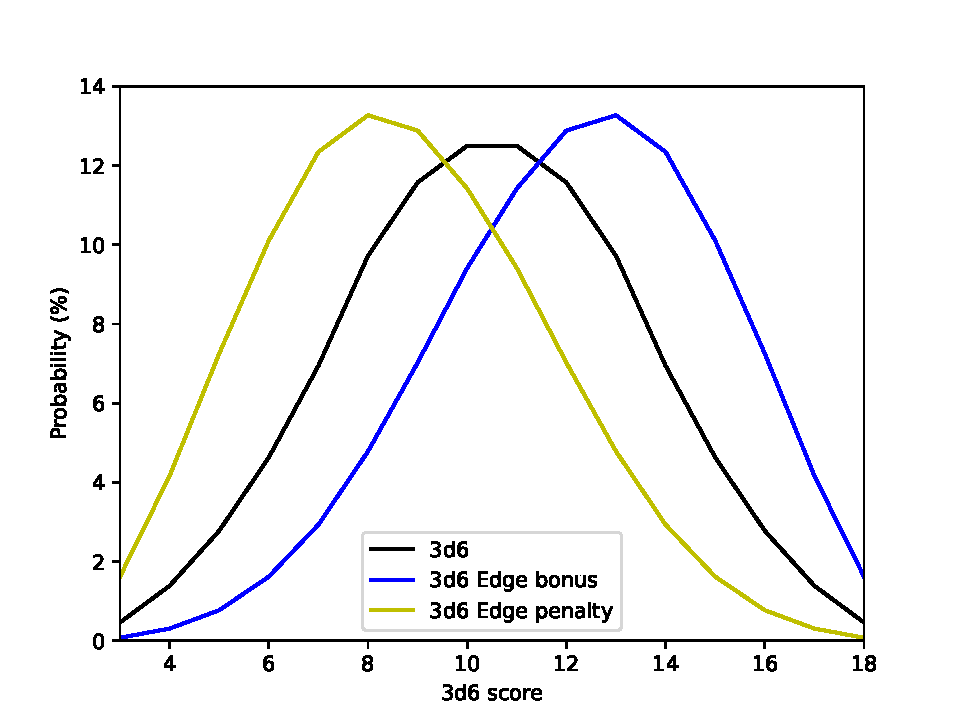
\includegraphics{prob_distribution_3d6.pdf}}
	\resizebox{0.49\hsize}{!}{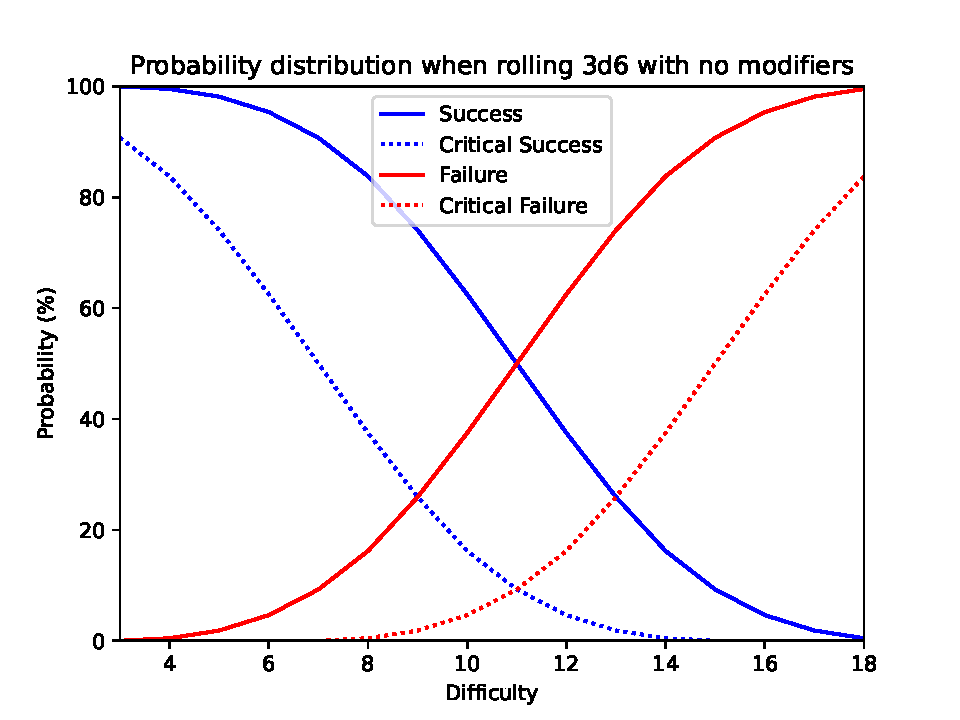
\includegraphics{success_distribution_3d6.pdf}}
	\caption{Left: the probability distribution for scores on 3d6. Right: chances of success and failure for different difficulties on 3d6. } 
\end{figure}

\end{appendices}


\end{document}